%%
%% Automatically generated file from DocOnce source
%% (https://github.com/hplgit/doconce/)
%%

% #define PREAMBLE

% #ifdef PREAMBLE
%-------------------- begin preamble ----------------------

\documentclass[%
oneside,                 % oneside: electronic viewing, twoside: printing
final,                   % draft: marks overfull hboxes, figures with paths
10pt]{article}

\listfiles               % print all files needed to compile this document

\usepackage{relsize,makeidx,color,setspace,amsmath,amsfonts,amssymb}
\usepackage[table]{xcolor}
\usepackage{bm,microtype}

\usepackage[pdftex]{graphicx}

% Packages for typesetting blocks of computer code
\usepackage{fancyvrb,framed,moreverb}

% Define colors
\definecolor{orange}{cmyk}{0,0.4,0.8,0.2}
\definecolor{tucorange}{rgb}{1.0,0.64,0}
\definecolor{darkorange}{rgb}{.71,0.21,0.01}
\definecolor{darkgreen}{rgb}{.12,.54,.11}
\definecolor{myteal}{rgb}{.26, .44, .56}
\definecolor{gray}{gray}{0.45}
\definecolor{mediumgray}{gray}{.8}
\definecolor{lightgray}{gray}{.95}
\definecolor{brown}{rgb}{0.54,0.27,0.07}
\definecolor{purple}{rgb}{0.5,0.0,0.5}
\definecolor{darkgray}{gray}{0.25}
\definecolor{darkblue}{rgb}{0,0.08,0.45}
\definecolor{darkblue2}{rgb}{0,0,0.8}
\definecolor{lightred}{rgb}{1.0,0.39,0.28}
\definecolor{lightgreen}{rgb}{0.48,0.99,0.0}
\definecolor{lightblue}{rgb}{0.53,0.81,0.92}
\definecolor{lightblue2}{rgb}{0.3,0.3,1.0}
\definecolor{lightpurple}{rgb}{0.87,0.63,0.87}
\definecolor{lightcyan}{rgb}{0.5,1.0,0.83}

\colorlet{comment_green}{green!50!black}
\colorlet{string_red}{red!60!black}
\colorlet{keyword_pink}{magenta!70!black}
\colorlet{indendifier_green}{green!70!white}

% Backgrounds for code
\definecolor{cbg_gray}{rgb}{.95, .95, .95}
\definecolor{bar_gray}{rgb}{.92, .92, .92}

\definecolor{cbg_yellowgray}{rgb}{.95, .95, .85}
\definecolor{bar_yellowgray}{rgb}{.95, .95, .65}

\colorlet{cbg_yellow2}{yellow!10}
\colorlet{bar_yellow2}{yellow!20}

\definecolor{cbg_yellow1}{rgb}{.98, .98, 0.8}
\definecolor{bar_yellow1}{rgb}{.98, .98, 0.4}

\definecolor{cbg_red1}{rgb}{1, 0.85, 0.85}
\definecolor{bar_red1}{rgb}{1, 0.75, 0.85}

\definecolor{cbg_blue1}{rgb}{0.87843, 0.95686, 1.0}
\definecolor{bar_blue1}{rgb}{0.7,     0.95686, 1}

%\setlength{\fboxsep}{-1.5mm}  % adjust cod_vpad/pro_vpad background box

%% Background for code blocks (parameter is color name)

%% pro/cod_vpad: gives some vertical padding before and after the text
%% (but has more simplistic code than _cod/pro_tight+cod/pro).
%% pro/cod_vpad can be used to enclose Verbatim or lst begin/end for code.
%% pro/cod calls _pro/cod_tight and has very little vertical padding,
%% used to enclose Verbatim and other begin/end for code.
%% (pro/cod is what the ptex2tex program could produce with the
%% Blue/BlueBar definitions in .ptex2tex.cfg.)

\newenvironment{cod_vpad}[1]{
   \def\FrameCommand{\colorbox{#1}}
   \MakeFramed{\FrameRestore}}
   {\endMakeFramed}

\newenvironment{_cod_tight}[1]{
   \def\FrameCommand{\colorbox{#1}}
   \FrameRule0.6pt\MakeFramed {\FrameRestore}\vskip3mm}
   {\vskip0mm\endMakeFramed}

\newenvironment{cod}[1]{
\bgroup\rmfamily
\fboxsep=0mm\relax
\begin{_cod_tight}{#1}
\list{}{\parsep=-2mm\parskip=0mm\topsep=0pt\leftmargin=2mm
\rightmargin=2\leftmargin\leftmargin=4pt\relax}
\item\relax}
{\endlist\end{_cod_tight}\egroup}

%% Background for complete program blocks (parameter 1 is color name
%% for background, parameter 2 is color for left bar)
\newenvironment{pro_vpad}[2]{
   \def\FrameCommand{\color{#2}\vrule width 1mm\normalcolor\colorbox{#1}}
   \MakeFramed{\FrameRestore}}
   {\endMakeFramed}

\newenvironment{_pro_tight}[2]{
   \def\FrameCommand{\color{#2}\vrule width 1mm\normalcolor\colorbox{#1}}
   \FrameRule0.6pt\MakeFramed {\advance\hsize-2mm\FrameRestore}\vskip3mm}
   {\vskip0mm\endMakeFramed}

\newenvironment{pro}[2]{
\bgroup\rmfamily
\fboxsep=0mm\relax
\begin{_pro_tight}{#1}{#2}
\list{}{\parsep=-2mm\parskip=0mm\topsep=0pt\leftmargin=2mm
\rightmargin=2\leftmargin\leftmargin=4pt\relax}
\item\relax}
{\endlist\end{_pro_tight}\egroup}


\usepackage[T1]{fontenc}
%\usepackage[latin1]{inputenc}
\usepackage{ucs}
\usepackage[utf8x]{inputenc}

\usepackage{lmodern}         % Latin Modern fonts derived from Computer Modern

% Hyperlinks in PDF:
\definecolor{linkcolor}{rgb}{0,0,0.4}
\usepackage{hyperref}
\hypersetup{
    breaklinks=true,
    colorlinks=true,
    linkcolor=linkcolor,
    urlcolor=linkcolor,
    citecolor=black,
    filecolor=black,
    %filecolor=blue,
    pdfmenubar=true,
    pdftoolbar=true,
    bookmarksdepth=3   % Uncomment (and tweak) for PDF bookmarks with more levels than the TOC
    }
%\hyperbaseurl{}   % hyperlinks are relative to this root

\setcounter{tocdepth}{2}  % number chapter, section, subsection

% Tricks for having figures close to where they are defined:
% 1. define less restrictive rules for where to put figures
\setcounter{topnumber}{2}
\setcounter{bottomnumber}{2}
\setcounter{totalnumber}{4}
\renewcommand{\topfraction}{0.95}
\renewcommand{\bottomfraction}{0.95}
\renewcommand{\textfraction}{0}
\renewcommand{\floatpagefraction}{0.75}
% floatpagefraction must always be less than topfraction!
% 2. ensure all figures are flushed before next section
\usepackage[section]{placeins}
% 3. enable begin{figure}[H] (often leads to ugly pagebreaks)
%\usepackage{float}\restylefloat{figure}

\usepackage[framemethod=TikZ]{mdframed}

% --- begin definitions of admonition environments ---

% Admonition style "mdfbox" is an oval colored box based on mdframed
% "notice" admon
\colorlet{mdfbox_notice_background}{gray!5}
\newmdenv[
  skipabove=15pt,
  skipbelow=15pt,
  outerlinewidth=0,
  backgroundcolor=mdfbox_notice_background,
  linecolor=black,
  linewidth=2pt,       % frame thickness
  frametitlebackgroundcolor=blue!5,
  frametitlerule=true,
  frametitlefont=\normalfont\bfseries,
  shadow=false,        % frame shadow?
  shadowsize=11pt,
  leftmargin=0,
  rightmargin=0,
  roundcorner=5,
  needspace=0pt,
]{notice_mdfboxmdframed}

\newenvironment{notice_mdfboxadmon}[1][]{
\begin{notice_mdfboxmdframed}[frametitle=#1]
}
{
\end{notice_mdfboxmdframed}
}

% Admonition style "mdfbox" is an oval colored box based on mdframed
% "summary" admon
\colorlet{mdfbox_summary_background}{gray!5}
\newmdenv[
  skipabove=15pt,
  skipbelow=15pt,
  outerlinewidth=0,
  backgroundcolor=mdfbox_summary_background,
  linecolor=black,
  linewidth=2pt,       % frame thickness
  frametitlebackgroundcolor=blue!5,
  frametitlerule=true,
  frametitlefont=\normalfont\bfseries,
  shadow=false,        % frame shadow?
  shadowsize=11pt,
  leftmargin=0,
  rightmargin=0,
  roundcorner=5,
  needspace=0pt,
]{summary_mdfboxmdframed}

\newenvironment{summary_mdfboxadmon}[1][]{
\begin{summary_mdfboxmdframed}[frametitle=#1]
}
{
\end{summary_mdfboxmdframed}
}

% Admonition style "mdfbox" is an oval colored box based on mdframed
% "warning" admon
\colorlet{mdfbox_warning_background}{gray!5}
\newmdenv[
  skipabove=15pt,
  skipbelow=15pt,
  outerlinewidth=0,
  backgroundcolor=mdfbox_warning_background,
  linecolor=black,
  linewidth=2pt,       % frame thickness
  frametitlebackgroundcolor=blue!5,
  frametitlerule=true,
  frametitlefont=\normalfont\bfseries,
  shadow=false,        % frame shadow?
  shadowsize=11pt,
  leftmargin=0,
  rightmargin=0,
  roundcorner=5,
  needspace=0pt,
]{warning_mdfboxmdframed}

\newenvironment{warning_mdfboxadmon}[1][]{
\begin{warning_mdfboxmdframed}[frametitle=#1]
}
{
\end{warning_mdfboxmdframed}
}

% Admonition style "mdfbox" is an oval colored box based on mdframed
% "question" admon
\colorlet{mdfbox_question_background}{gray!5}
\newmdenv[
  skipabove=15pt,
  skipbelow=15pt,
  outerlinewidth=0,
  backgroundcolor=mdfbox_question_background,
  linecolor=black,
  linewidth=2pt,       % frame thickness
  frametitlebackgroundcolor=blue!5,
  frametitlerule=true,
  frametitlefont=\normalfont\bfseries,
  shadow=false,        % frame shadow?
  shadowsize=11pt,
  leftmargin=0,
  rightmargin=0,
  roundcorner=5,
  needspace=0pt,
]{question_mdfboxmdframed}

\newenvironment{question_mdfboxadmon}[1][]{
\begin{question_mdfboxmdframed}[frametitle=#1]
}
{
\end{question_mdfboxmdframed}
}

% Admonition style "mdfbox" is an oval colored box based on mdframed
% "block" admon
\colorlet{mdfbox_block_background}{gray!5}
\newmdenv[
  skipabove=15pt,
  skipbelow=15pt,
  outerlinewidth=0,
  backgroundcolor=mdfbox_block_background,
  linecolor=black,
  linewidth=2pt,       % frame thickness
  frametitlebackgroundcolor=blue!5,
  frametitlerule=true,
  frametitlefont=\normalfont\bfseries,
  shadow=false,        % frame shadow?
  shadowsize=11pt,
  leftmargin=0,
  rightmargin=0,
  roundcorner=5,
  needspace=0pt,
]{block_mdfboxmdframed}

\newenvironment{block_mdfboxadmon}[1][]{
\begin{block_mdfboxmdframed}[frametitle=#1]
}
{
\end{block_mdfboxmdframed}
}

% --- end of definitions of admonition environments ---

% prevent orhpans and widows
\clubpenalty = 10000
\widowpenalty = 10000

\newenvironment{doconceexercise}{}{}
\newcounter{doconceexercisecounter}
% --- begin definition of \listofexercises command ---
\makeatletter
\newcommand\listofexercises{\section*{List of Exercises and Problems}
\@starttoc{loe}
}
\newcommand*{\l@doconceexercise}{\@dottedtocline{0}{0pt}{6.5em}}
\makeatother
% --- end definition of \listofexercises command ---



% ------ header in subexercises ------
%\newcommand{\subex}[1]{\paragraph{#1}}
%\newcommand{\subex}[1]{\par\vspace{1.7mm}\noindent{\bf #1}\ \ }
\makeatletter
% 1.5ex is the spacing above the header, 0.5em the spacing after subex title
\newcommand\subex{\@startsection{paragraph}{4}{\z@}%
                  {1.5ex\@plus1ex \@minus.2ex}%
                  {-0.5em}%
                  {\normalfont\normalsize\bfseries}}
\makeatother


% --- end of standard preamble for documents ---


% insert custom LaTeX commands...

\raggedbottom
\makeindex
\usepackage[totoc]{idxlayout}   % for index in the toc
\usepackage[nottoc]{tocbibind}  % for references/bibliography in the toc

%-------------------- end preamble ----------------------

\begin{document}

% matching end for #ifdef PREAMBLE
% #endif

\newcommand{\half}{\frac{1}{2}}
\newcommand{\halfi}{{1/2}}
\newcommand{\tp}{\thinspace .}

\newcommand{\uex}{{u_{\small\mbox{e}}}}
\newcommand{\uexd}[1]{{u_{\small\mbox{e}, #1}}}
\newcommand{\vex}{{v_{\small\mbox{e}}}}
\newcommand{\vexd}[1]{{v_{\small\mbox{e}, #1}}}
\newcommand{\Aex}{{A_{\small\mbox{e}}}}

% Operators
\newcommand{\Ddt}[1]{\frac{D #1}{dt}}
\newcommand{\E}[1]{\hbox{E}\lbrack #1 \rbrack}
\newcommand{\Var}[1]{\hbox{Var}\lbrack #1 \rbrack}
\newcommand{\Std}[1]{\hbox{Std}\lbrack #1 \rbrack}

\newcommand{\xpoint}{\bm{x}}
\newcommand{\normalvec}{\bm{n}}
\newcommand{\Oof}[1]{\mathcal{O}(#1)}

% Boldface vectors/tensors
\newcommand{\x}{\bm{x}}
\newcommand{\X}{\bm{X}}
\renewcommand{\u}{\bm{u}}
\renewcommand{\v}{\bm{v}}
\newcommand{\w}{\bm{w}}
\newcommand{\acc}{\bm{a}}
\newcommand{\rpos}{\bm{r}}
\newcommand{\V}{\bm{V}}
\newcommand{\e}{\bm{e}}
\newcommand{\f}{\bm{f}}
\newcommand{\F}{\bm{F}}
\newcommand{\stress}{\bm{\sigma}}
\newcommand{\strain}{\bm{\varepsilon}}
\newcommand{\stressc}{{\sigma}}
\newcommand{\strainc}{{\varepsilon}}
\newcommand{\I}{\bm{I}}
\newcommand{\T}{\bm{T}}

\newcommand{\dfc}{\alpha}  % diffusion coefficient
% Unit vectors
\newcommand{\ii}{\bm{i}}
\newcommand{\jj}{\bm{j}}
\newcommand{\kk}{\bm{k}}
\newcommand{\ir}{\bm{i}_r}
\newcommand{\ith}{\bm{i}_{\theta}}
\newcommand{\iz}{\bm{i}_z}

% Index sets
\newcommand{\Ix}{\mathcal{I}_x}
\newcommand{\Iy}{\mathcal{I}_y}
\newcommand{\Iz}{\mathcal{I}_z}
\newcommand{\It}{\mathcal{I}_t}
%\newcommand{\Ix}{{I_x}}
%\newcommand{\Iy}{{I_y}}
%\newcommand{\Iz}{{I_z}}
%\newcommand{\It}{{I_t}}
%\newcommand{\If}{\mathcal{I}}     % for FEM
\newcommand{\If}{\mathcal{I}_s}     % for FEM
%\newcommand{\If}{{I}}     % for FEM
%\newcommand{\Ifd}{\mathcal{I}_d}  % for FEM
\newcommand{\Ifd}{{I_d}}  % for FEM
\newcommand{\Ifb}{{I_b}}  % for FEM
\newcommand{\setb}[1]{#1^0}    % set begin
\newcommand{\sete}[1]{#1^{-1}} % set end
%\newcommand{\setl}[1]{#1\setminus\{\set1{#1}\}}
%\newcommand{\setr}[1]{#1\setminus\{\set0{#1}\}}
%\newcommand{\seti}[1]{#1\setminus\{\set0{#1},\set1{#1}\}}
\newcommand{\setl}[1]{#1^-}
\newcommand{\setr}[1]{#1^+}
\newcommand{\seti}[1]{#1^i}
\newcommand{\sequencei}[1]{\left\{ {#1}_i \right\}_{i\in\If}}

% Finite elements
\newcommand{\basphi}{\varphi}
\newcommand{\baspsi}{\psi}
\newcommand{\refphi}{\tilde\basphi}
\newcommand{\psib}{\bm{\psi}}
\newcommand{\sinL}[1]{\sin\left((#1+1)\pi\frac{x}{L}\right)}
\newcommand{\xno}[1]{x_{#1}}
%\newcommand{\xno}[1]{x^{(#1)}}
\newcommand{\Xno}[1]{X_{(#1)}}
\newcommand{\yno}[1]{y_{#1}}
\newcommand{\Yno}[1]{Y_{(#1)}}
\newcommand{\xdno}[1]{\bm{x}_{#1}}

% FEniCS commands
\newcommand{\dX}{\, \mathrm{d}X}
\newcommand{\dx}{\, \mathrm{d}x}
\newcommand{\ds}{\, \mathrm{d}s}
\newcommand{\Real}{\mathbb{R}}
\newcommand{\Integerp}{\mathbb{N}}
\newcommand{\Integer}{\mathbb{Z}}


% ------------------- main content ----------------------



% ----------------- title -------------------------

\thispagestyle{empty}

\begin{center}
{\LARGE\bf
\begin{spacing}{1.25}
Software engineering with exponential decay models
\end{spacing}
}
\end{center}

% ----------------- author(s) -------------------------

\begin{center}
{\bf Hans Petter Langtangen${}^{1, 2}$} \\ [0mm]
\end{center}

\begin{center}
% List of all institutions:
\centerline{{\small ${}^1$Center for Biomedical Computing, Simula Research Laboratory}}
\centerline{{\small ${}^2$Department of Informatics, University of Oslo}}
\end{center}
    
% ----------------- end author(s) -------------------------

% --- begin date ---
\begin{center}
Oct 10, 2015
\end{center}
% --- end date ---

\vspace{1cm}


\tableofcontents

\clearpage % pagebreak before list of exercises
\subsection*{List of Exercises and Problems}
\begin{tabular}{lrll}
Problem & 1 & Make a tool for differentiating curves & p.~\pageref{softeng1:exer:derivative} \\
Problem & 2 & Make solid software for the Trapezoidal rule & p.~\pageref{softeng1:exer:integral:flat} \\
Problem & 3 & Implement classes for the Trapezoidal rule & p.~\pageref{softeng1:exer:integral:flat2} \\
Problem & 4 & Write a doctest and a test function & p.~\pageref{softeng1:exer:doctest1} \\
Problem & 5 & Experiment with tolerances in comparisons & p.~\pageref{softeng1:exer:tol} \\
Exercise & 6 & Make use of a class implementation & p.~\pageref{softeng1:exer:class:dts} \\
Problem & 7 & Make solid software for a difference equation & p.~\pageref{softeng1:exer:logistic} \\
\end{tabular}
% --- end of table of exercises
\clearpage % pagebreak after list of exercises




\vspace{1cm} % after toc







% !split

Teaching material on scientific computing has traditionally been very
focused on the mathematics and the applications, while details on how
the computer is programmed to solve the problems have received little attention.
Many end up writing as simple programs as possible, without being
aware of much useful computer science technology that would increase
the fun, efficiency, and reliability of the their scientific computing
activities.

This chapter demonstrates a series of good practices and tools
from modern computer science, using the simple mathematical problem
$u^{\prime}=-au$, $u(0)=I$, such that we minimize the
mathematical details and can go more in depth with implementations.
The goal is to increase the technological
quality of computer programming and make it match the more
well-established quality of the mathematics of scientific computing.

The conventions and techniques outlined here will save you a lot of time
when you incrementally extend software over time from simpler to more
complicated problems. In particular, you will benefit from
many good habits:

\begin{itemize}
 \item new code is added in a modular fashion to a library (modules),

 \item programs are run through convenient user interfaces,

 \item it takes one quick command to let all your code undergo heavy testing,

 \item tedious manual work with running programs is automated,

 \item your scientific investigations are reproducible,

 \item scientific reports with top quality typesetting are produced both
   for paper and electronic devices.
\end{itemize}

\noindent
\section{Implementations with functions and modules}
\label{softeng1:basic}

All previous examples in this book have implemented numerical
algorithms as Python functions. This is a good style that readers
are expected to adopt. However, this author has experienced that
many students and engineers are inclined to make ``flat'' programs,
i.e., a sequence of statements without any use of functions, just to
get the problem solved as quickly as possible. Since this programming
style is so widespread, especially among people with MATLAB experience,
we shall look at the weaknesses of flat programs and show how they
can be \emph{refactored} into more reusable programs based on functions.

\subsection{Mathematical problem and solution technique}
\label{softeng1:basic:math}

We address the differential equation problem

\begin{align}
u'(t) &= -au(t), \quad t \in (0,T], \label{softeng1:ode}\\ 
u(0)  &= I,                         \label{softeng1:u0}
\end{align}
where $a$, $I$, and $T$ are prescribed parameters, and $u(t)$ is
the unknown function to be estimated. This mathematical model
is relevant for physical phenomena featuring exponential decay
in time, e.g., vertical pressure variation in the atmosphere,
cooling of an object, and radioactive decay.

The
time domain is discretized with points $0 = t_0 < t_1 \cdots < t_{N_t}=T$,
here with a constant spacing $\Delta t$ between the
mesh points: $\Delta t = t_{n}-t_{n-1}$, $n=1,\ldots,N_t$. Let
$u^n$ be the numerical approximation to the exact solution at $t_n$.
A family of popular numerical methods are provided by the $\theta$ scheme,

\begin{equation}
u^{n+1} = \frac{1 - (1-\theta) a\Delta t}{1 + \theta a\Delta t}u^n,
\label{softeng1:utheta}
\end{equation}
for $n=0,1,\ldots,N_t-1$. This formula produces
the Forward Euler
scheme when $\theta=0$,
the Backward Euler
scheme when $\theta=1$,
and the Crank-Nicolson
scheme when $\theta=1/2$.


\subsection{A first, quick implementation}
\label{softeng1:basic:impl1}

Solving (\ref{softeng1:utheta}) in a program is very straightforward:
just make a loop over $n$ and evaluate the formula. The $u(t_n$)
values for discrete $n$ can be stored in an array. This makes it easy
to also plot the solution. It would be natural to also add
the exact
solution curve $u(t)=Ie^{-at}$ to the plot.

Many have programming habits that would lead them
to write a simple program like this:

\begin{pro}{cbg_blue1}{bar_blue1}\begin{Verbatim}[numbers=none,fontsize=\fontsize{9pt}{9pt},baselinestretch=0.95,xleftmargin=2mm]
from numpy import *
from matplotlib.pyplot import *

A = 1
a = 2
T = 4
dt = 0.2
N = int(round(T/dt))
y = zeros(N+1)
t = linspace(0, T, N+1)
theta = 1
y[0] = A
for n in range(0, N):
    y[n+1] = (1 - (1-theta)*a*dt)/(1 + theta*dt*a)*y[n]

y_e = A*exp(-a*t) - y
error = y_e - y
E = sqrt(dt*sum(error**2))
print 'Norm of the error: %.3E' % E
plot(t, y, 'r--o')
t_e = linspace(0, T, 1001)
y_e = A*exp(-a*t_e)
plot(t_e, y_e, 'b-')
legend(['numerical, theta=%g' % theta, 'exact'])
xlabel('t')
ylabel('y')
show()
\end{Verbatim}
\end{pro}
\noindent

This program is easy to read, and as long as it is correct, many will
claim that it has sufficient quality. Nevertheless, the program suffers
from two serious flaws:

\begin{enumerate}
\item The notation in the program does not correspond \emph{exactly} to
   the notation in the mathematical problem: the solution is called
   \texttt{y} and corresponds to $u$ in the mathematical description,
   the variable \texttt{A} corresponds to the mathematical parameter $I$,
   \texttt{N} in the program is called $N_t$ in the mathematics.

\item There are no comments in the program.
\end{enumerate}

\noindent
These kind of flaws quickly become crucial if present in code for complicated
mathematical problems and code that is meant to be extended to other problems.

We also note that the program is \emph{flat} in the sense that it does
not contain functions. Usually, this is a bad habit, but let us
first correct the two mentioned flaws.

\subsection{A more decent program}
\label{softeng1:basic:impl2}

A code of better quality arises from
fixing the notation and adding comments:

\begin{pro}{cbg_blue1}{bar_blue1}\begin{Verbatim}[numbers=none,fontsize=\fontsize{9pt}{9pt},baselinestretch=0.95,xleftmargin=2mm]
from numpy import *
from matplotlib.pyplot import *

I = 1
a = 2
T = 4
dt = 0.2
Nt = int(round(T/dt))     # no of time intervals
u = zeros(Nt+1)           # array of u[n] values
t = linspace(0, T, Nt+1)  # time mesh
theta = 1                 # Backward Euler method

u[0] = I                  # assign initial condition
for n in range(0, Nt):    # n=0,1,...,Nt-1
    u[n+1] = (1 - (1-theta)*a*dt)/(1 + theta*dt*a)*u[n]

# Compute norm of the error
u_e = I*exp(-a*t) - u     # exact u at the mesh points
error = u_e - u
E = sqrt(dt*sum(error**2))
print 'Norm of the error: %.3E' % E

# Compare numerical (u) and exact solution (u_e) in a plot
plot(t, u, 'r--o')
t_e = linspace(0, T, 1001)       # very fine mesh for u_e
u_e = I*exp(-a*t_e)
plot(t_e, u_e, 'b-')
legend(['numerical, theta=%g' % theta, 'exact'])
xlabel('t')
ylabel('u')
show()
\end{Verbatim}
\end{pro}
\noindent

\paragraph{Comments in a program.}
There is obviously not just one way to comment a program, and opinions
may differ as to what code should be commented.
The guiding principle is, however, that comments should make the
program easy to understand for the human eye. Do not comment obvious
constructions, but focus on ideas and (``what happens in the next
statements?'') and on explaining code that can be found
complicated.


\index{refactoring}

\paragraph{Refactoring into functions.}
At first sight, our updated program seems like
a good starting point for playing around
with the mathematical problem: we can just change parameters and rerun.
Although such edit-and-rerun sessions are good for initial exploration,
one will soon extend the experiments and start developing the code
further. Say we want to compare $\theta =0,1,0.5$ in the same
plot. This extension requires changes all over the code and quickly
leads to errors. To do something serious with this program, we have to
break it into smaller pieces and make sure each piece is well tested,
and ensure that the program is sufficiently general and can be reused in
new contexts without changes.  The
next natural step is therefore to isolate the numerical computations
and the visualization in separate Python functions.
Such a rewrite of a code, without essentially changing the functionality,
but just improve the quality of the code, is known as \emph{refactoring}.
After quickly putting together and testing a program, the next
step is to refactor it so it becomes better prepared for extensions.

\paragraph{Program file vs IDE vs notebook.}
There are basically three different ways of working with Python code:

\begin{enumerate}
\item One writes the code in a file, using a text editor (such as
   Emacs or Vim) and runs it in a terminal window.

\item One applies an \emph{Integrated Development Environment} (the simplest is IDLE, which comes with standard Python) containing a graphical user interface with an editor and an element where Python code can be run.

\item One applies the Jupyter Notebook (previously known as IPython Notebook),
   which offers an interactive environment for Python code where
   plots are automatically inserted after the code, see Figure~\ref{softeng1:ipynb}.
\end{enumerate}

\noindent
It appears that method 1 and 2 are quite equivalent, but the notebook
encourages more experimental code and therefore also flat programs.
Consequently, notebook users will normally need to think more about
refactoring code and increase the use of functions after initial
experimentation.


\begin{figure}[!ht]  % softeng1:ipynb
  \centerline{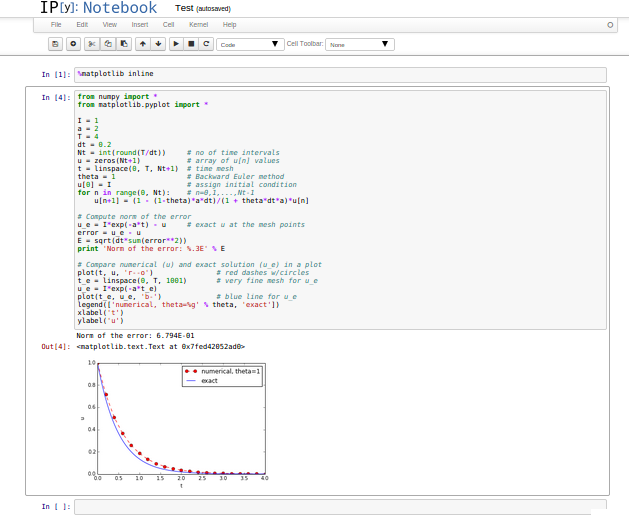
\includegraphics[width=0.8\linewidth]{fig-softeng/ipynb_flat.png}}
  \caption{
  Experimental code in a notebook. \label{softeng1:ipynb}
  }
\end{figure}
%\clearpage % flush figures softeng1:ipynb



\subsection{Prefixing imported functions by the module name}
\label{softeng1:basic:modprefix}

\index{importing modules}

Import statements of the form \texttt{from module import *} import
\emph{all} functions and variables in \texttt{module.py} into the current file.
This is often referred to as ``import star'', and
many find this convenient, but it is not considered as a good
programming style in Python.
For example, when doing

\begin{cod}{cbg_blue1}\begin{Verbatim}[numbers=none,fontsize=\fontsize{9pt}{9pt},baselinestretch=0.95,xleftmargin=2mm]
from numpy import *
from matplotlib.pyplot import *
\end{Verbatim}
\end{cod}
\noindent
we get mathematical functions like \texttt{sin} and \texttt{exp} as well as
MATLAB-style functions like \texttt{linspace} and \texttt{plot}, which can be called
by these well-known names.  Unfortunately, it sometimes becomes
confusing to know where a particular function comes from, i.e., what
modules you need to import. Is a desired function from \texttt{numpy} or
\texttt{matplotlib.pyplot}? Or is it our own function?  These questions are
easy to answer if functions in modules are prefixed by the module
name. Doing an additional \texttt{from math import *} is really crucial: now
\texttt{sin}, \texttt{cos}, and other mathematical functions are imported and their
names hide those previously imported from \texttt{numpy}.  That is, \texttt{sin} is
now a sine function that accepts a \texttt{float} argument, not an array.

Doing the import such that module functions must have a prefix
is generally recommended:

\begin{cod}{cbg_blue1}\begin{Verbatim}[numbers=none,fontsize=\fontsize{9pt}{9pt},baselinestretch=0.95,xleftmargin=2mm]
import numpy
import matplotlib.pyplot

t = numpy.linspace(0, T, Nt+1)
u_e = I*numpy.exp(-a*t)
matplotlib.pyplot.plot(t, u_e)
\end{Verbatim}
\end{cod}
\noindent

The modules \texttt{numpy} and \texttt{matplotlib.pyplot} are frequently used,
and since their full names are quite tedious to write,
two standard abbreviations
have evolved in the Python scientific computing community:

\begin{cod}{cbg_blue1}\begin{Verbatim}[numbers=none,fontsize=\fontsize{9pt}{9pt},baselinestretch=0.95,xleftmargin=2mm]
import numpy as np
import matplotlib.pyplot as plt

t = np.linspace(0, T, Nt+1)
u_e = I*np.exp(-a*t)
plt.plot(t, u_e)
\end{Verbatim}
\end{cod}
\noindent

The downside of prefixing functions by the module name is that
mathematical expressions like $e^{-at}\sin(2\pi t)$ get
cluttered with module names,
\begin{cod}{cbg_blue1}\begin{Verbatim}[numbers=none,fontsize=\fontsize{9pt}{9pt},baselinestretch=0.95,xleftmargin=2mm]
numpy.exp(-a*t)*numpy.sin(2(numpy.pi*t)
# or
np.exp(-a*t)*np.sin(2*np.pi*t)
\end{Verbatim}
\end{cod}
\noindent
Such an expression looks like \texttt{exp(-a*t)*sin(2*pi*t)} in most other
programming languages. Similarly, \texttt{np.linspace} and \texttt{plt.plot} look
less familiar to people who are used to MATLAB and who have not
adopted Python's prefix style.  Whether to do \texttt{from module import *}
or \texttt{import module} depends on personal taste and the problem at
hand. In these writings we use \texttt{from module import *} in more basic,
shorter programs where similarity with MATLAB could be an
advantage. However, in reusable modules we prefix calls to module
functions by their function name, \emph{or} do explicit import of the
needed functions:

\begin{cod}{cbg_blue1}\begin{Verbatim}[numbers=none,fontsize=\fontsize{9pt}{9pt},baselinestretch=0.95,xleftmargin=2mm]
from numpy import exp, sum, sqrt

def u_exact(t, I, a):
    return I*exp(-a*t)

error = u_exact(t, I, a) - u
E = sqrt(dt*sum(error**2))
\end{Verbatim}
\end{cod}
\noindent


\begin{notice_mdfboxadmon}[Prefixing module functions or not?]
It can be advantageous to do a combination: mathematical functions
in formulas are imported without prefix, while module functions
in general are called with a prefix. For the \texttt{numpy} package we
can do

\begin{cod}{cbg_blue1}\begin{Verbatim}[numbers=none,fontsize=\fontsize{9pt}{9pt},baselinestretch=0.95,xleftmargin=2mm]
import numpy as np
from numpy import exp, sum, sqrt
\end{Verbatim}
\end{cod}
\noindent
such that mathematical expression can apply \texttt{exp}, \texttt{sum}, and \texttt{sqrt}
and hence look as close to the mathematical formulas as possible
(without a disturbing prefix).
Other calls to \texttt{numpy} function are done with the prefix, as in
\texttt{np.linspace}.
\end{notice_mdfboxadmon}




\subsection{Implementing the numerical algorithm in a function}
\label{softeng1:basic:func}

The solution formula (\ref{softeng1:utheta}) is completely general and
should be available as a Python function \texttt{solver} with all input data as
function arguments and all output data returned to the calling code.
With this \texttt{solver} function we can solve all types of problems
(\ref{softeng1:ode})-(\ref{softeng1:u0})
by an easy-to-read one-line statement:

\begin{cod}{cbg_blue1}\begin{Verbatim}[numbers=none,fontsize=\fontsize{9pt}{9pt},baselinestretch=0.95,xleftmargin=2mm]
u, t = solver(I=1, a=2, T=4, dt=0.2, theta=0.5)
\end{Verbatim}
\end{cod}
\noindent

Refactoring the numerical method in the previous flat program
in terms of a \texttt{solver} function and prefixing calls to
module functions by the module name leads to this code:

\begin{cod}{cbg_blue1}\begin{Verbatim}[numbers=none,fontsize=\fontsize{9pt}{9pt},baselinestretch=0.95,xleftmargin=2mm]
def solver(I, a, T, dt, theta):
    """Solve u'=-a*u, u(0)=I, for t in (0,T] with steps of dt."""
    dt = float(dt)               # avoid integer division
    Nt = int(round(T/dt))        # no of time intervals
    T = Nt*dt                    # adjust T to fit time step dt
    u = np.zeros(Nt+1)           # array of u[n] values
    t = np.linspace(0, T, Nt+1)  # time mesh

    u[0] = I                  # assign initial condition
    for n in range(0, Nt):    # n=0,1,...,Nt-1
        u[n+1] = (1 - (1-theta)*a*dt)/(1 + theta*dt*a)*u[n]
    return u, t
\end{Verbatim}
\end{cod}
\noindent


\begin{notice_mdfboxadmon}[Tip: Always use a doc string to document a function!]
Python has a convention for documenting the purpose and usage of
a function in a \emph{doc string}: simply place the documentation
in a one- or multi-line triple-quoted string right after the
function header.
\end{notice_mdfboxadmon}




\begin{notice_mdfboxadmon}[Be careful with unintended integer division!]
Note that we in the \texttt{solver} function explicitly covert \texttt{dt} to a
\texttt{float} object. If not, the updating formula for \texttt{u[n+1]} may evaluate
to zero because of integer division when \texttt{theta}, \texttt{a}, and \texttt{dt} are integers!
\end{notice_mdfboxadmon}



\subsection{Do not have several versions of a code}

One of the most serious flaws in computational work is to have several
slightly different implementations of the same computational algorithms
lying around in various program files. This is very likely to happen,
because busy scientists often want to test a slight variation of a code to see
what happens. A quick copy-and-edit does the task, but such quick hacks tend
to survive. When a real correction is needed in the implementation,
it is difficult to ensure that the correction is done in all relevant files.
In fact, this is a general problem in programming, which has led to
an important principle.


\begin{notice_mdfboxadmon}[The DRY principle: Don't repeat yourself!]
When implementing a particular functionality in a computer program, make sure
this functionality and its variations are implemented in just one piece
of code. That is, if you need to revise the implementation, there should be
\emph{one and only one} place to edit. It follows that you should never
duplicate code (don't repeat yourself!), and code snippets that are
similar should be factored into one piece (function) and parameterized (by
function arguments).
\end{notice_mdfboxadmon}



The DRY principle means that our \texttt{solver} function should not be
copied to a new file if we need some modifications. Instead, we
should try to extend \texttt{solver} such that the new and old needs are
met by a single function. Sometimes this process requires a new
refactoring, but having a numerical method in one and only one place
is a great advantage.

\subsection{Making a module}
\label{softeng1:basic:module}

As soon as you start making Python functions in a program, you should
make sure the program file fulfills the requirement of a module.
This means that you can import and reuse your functions in other
programs too. For example, if our \texttt{solver} function resides in a
module file \texttt{decay.py}, another program may reuse of the
function either by

\begin{cod}{cbg_blue1}\begin{Verbatim}[numbers=none,fontsize=\fontsize{9pt}{9pt},baselinestretch=0.95,xleftmargin=2mm]
from decay import solver
u, t = solver(I=1, a=2, T=4, dt=0.2, theta=0.5)
\end{Verbatim}
\end{cod}
\noindent
or by a slightly different import statement, combined with a subsequent
prefix of the function name by the name of the module:

\begin{cod}{cbg_blue1}\begin{Verbatim}[numbers=none,fontsize=\fontsize{9pt}{9pt},baselinestretch=0.95,xleftmargin=2mm]
import decay
u, t = decay.solver(I=1, a=2, T=4, dt=0.2, theta=0.5)
\end{Verbatim}
\end{cod}
\noindent

The requirements for a program file to also qualify for a module are simple:

\begin{enumerate}
\item The filename without \texttt{.py} must be a valid Python variable name.

\item The main program must be executed (through statements or
   a function call) in the \emph{test block}.
\end{enumerate}

\noindent
The \emph{test block} is normally placed at the end of a module file:

\begin{cod}{cbg_blue1}\begin{Verbatim}[numbers=none,fontsize=\fontsize{9pt}{9pt},baselinestretch=0.95,xleftmargin=2mm]
if __name__ == '__main__':
    # Statements
\end{Verbatim}
\end{cod}
\noindent
When the module file is executed as a stand-alone program, the if test
is true and the indented statements are run. If the module file
is imported, however, \Verb!__name__! equals the module name and the test block
is not executed.

To demonstrate the difference, consider the trivial module
file \texttt{hello.py} with one function and a call to this function as main program:

\begin{pro}{cbg_blue1}{bar_blue1}\begin{Verbatim}[numbers=none,fontsize=\fontsize{9pt}{9pt},baselinestretch=0.95,xleftmargin=2mm]
def hello(arg='World!'):
    print 'Hello, ' + arg

if __name__ == '__main__':
    hello()
\end{Verbatim}
\end{pro}
\noindent
Without the test block, the code reads

\begin{pro}{cbg_blue1}{bar_blue1}\begin{Verbatim}[numbers=none,fontsize=\fontsize{9pt}{9pt},baselinestretch=0.95,xleftmargin=2mm]
def hello(arg='World!'):
    print 'Hello, ' + arg

hello()
\end{Verbatim}
\end{pro}
\noindent
With this latter version of the file, any attempt to import \texttt{hello}
will, at the same time, execute the call \texttt{hello()} and hence write
``Hello, World!'' to the screen.  Such output is not desired when
importing a module!  To make import and execution of code independent
for another program that wants to use the function \texttt{hello}, the module
\texttt{hello} must be written with a test block. Furthermore, running the
file itself as \texttt{python hello.py} will make the block active and lead
to the desired printing.


\begin{notice_mdfboxadmon}[All coming functions are placed in a module!]
The many functions to be explained in the following text are
put in one module file \href{{http://tinyurl.com/ofkw6kc/softeng/decay.py}}{\nolinkurl{decay.py}}.
\end{notice_mdfboxadmon}



What more than the \texttt{solver} function is needed in our \texttt{decay} module
to do everything we did in the previous, flat program?  We need import
statements for \texttt{numpy} and \texttt{matplotlib} as well as another function
for producing the plot. It can also be convenient to put the exact
solution in a Python function.  Our module \texttt{decay.py} then looks like
this:

\begin{cod}{cbg_blue1}\begin{Verbatim}[numbers=none,fontsize=\fontsize{9pt}{9pt},baselinestretch=0.95,xleftmargin=2mm]
import numpy as np
import matplotlib.pyplot as plt

def solver(I, a, T, dt, theta):
    ...

def u_exact(t, I, a):
    return I*np.exp(-a*t)

def experiment_compare_numerical_and_exact():
    I = 1;  a = 2;  T = 4;  dt = 0.4;  theta = 1
    u, t = solver(I, a, T, dt, theta)

    t_e = np.linspace(0, T, 1001)       # very fine mesh for u_e
    u_e = u_exact(t_e, I, a)

    plt.plot(t,   u,   'r--o')       # dashed red line with circles
    plt.plot(t_e, u_e, 'b-')         # blue line for u_e
    plt.legend(['numerical, theta=%g' % theta, 'exact'])
    plt.xlabel('t')
    plt.ylabel('u')
    plotfile = 'tmp'
    plt.savefig(plotfile + '.png');  plt.savefig(plotfile + '.pdf')

    error = u_exact(t, I, a) - u
    E = np.sqrt(dt*np.sum(error**2))
    print 'Error norm:', E

if __name__ == '__main__':
    experiment_compare_numerical_and_exact()
\end{Verbatim}
\end{cod}
\noindent
We could consider doing \texttt{from numpy import exp, sqrt, sum} to make
the mathematical expressions with these functions closer to the
mathematical formulas, but here we employed the prefix since the
formulas are so simple and easy to read.

This module file does exactly the same as the previous, flat program,
but now it becomes much easier to extend the code with more functions
that produce other plots, other experiments, etc. Even more important, though,
is that the numerical
algorithm is coded and tested once and for all in the \texttt{solver}
function, and any need to solve the mathematical problem is a matter
of one function call.
% (not copying initialization statements and a loop
% to a new program for ad hoc editing!).


\subsection{Example on extending the module code}
\label{softeng1:basic:experiment2}

Let us specifically demonstrate one extension of the flat program in
Section~\ref{softeng1:basic:impl1} that would require substantial
editing of the flat code (Section~\ref{softeng1:basic:impl2}), while in
a structured module (Section~\ref{softeng1:basic:module}), we can
simply add a new function without affecting the existing code.

Our example that illustrates the extension
is to make a comparison between the numerical solutions
for various schemes ($\theta$ values) and the exact solution:



% inline figure
\centerline{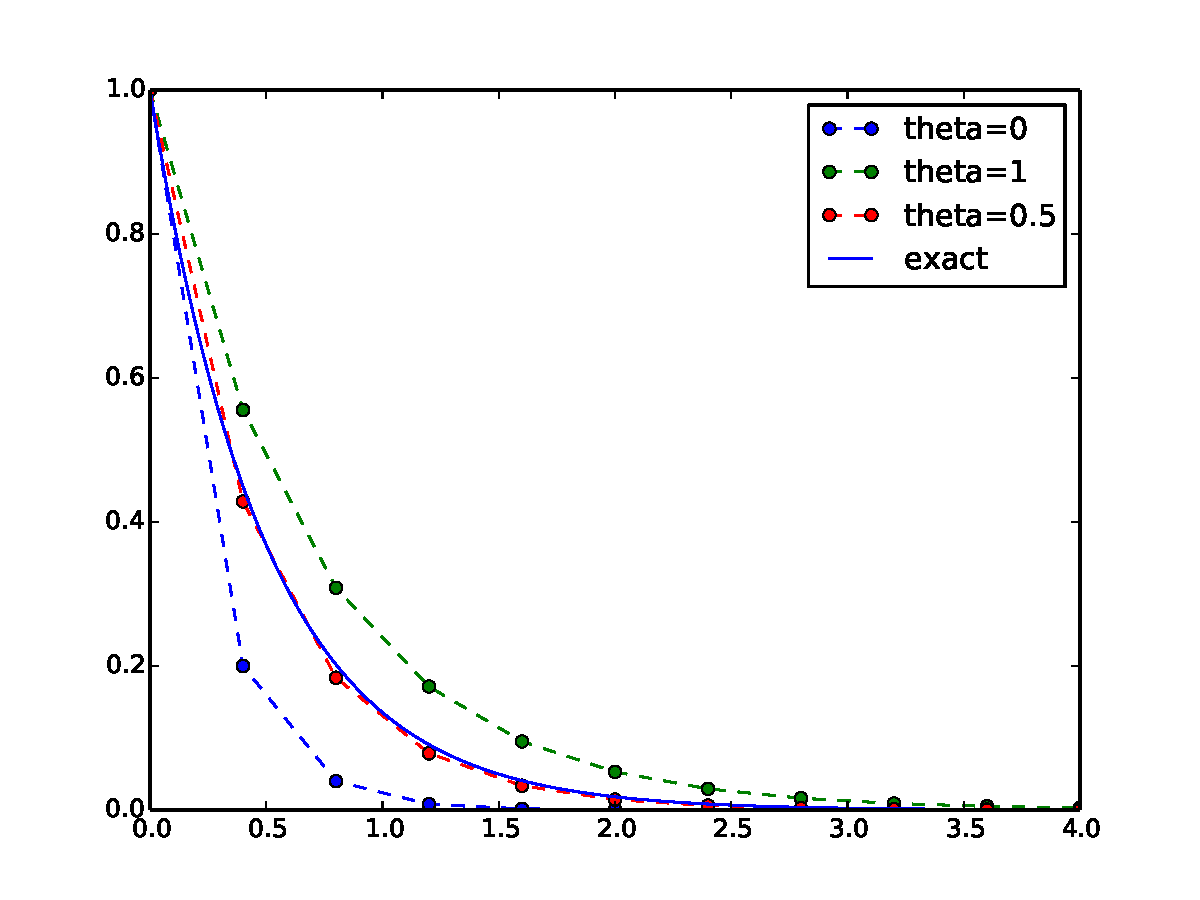
\includegraphics[width=0.7\linewidth]{fig-softeng/compare.pdf}}




\begin{question_mdfboxadmon}[Wait a minute!]
Look at the flat program in
Section~\ref{softeng1:basic:impl1},
and try to imagine which edits that are required to solve this new problem.
\end{question_mdfboxadmon}



With the \texttt{solver} function at hand, we can simply create a function
with a loop over \texttt{theta} values and add the necessary plot statements:

\begin{cod}{cbg_blue1}\begin{Verbatim}[numbers=none,fontsize=\fontsize{9pt}{9pt},baselinestretch=0.95,xleftmargin=2mm]
def experiment_compare_schemes():
    """Compare theta=0,1,0.5 in the same plot."""
    I = 1;  a = 2;  T = 4;  dt = 0.4
    legends = []
    for theta in [0, 1, 0.5]:
        u, t = solver(I, a, T, dt, theta)
        plt.plot(t, u, '--o')
        legends.append('theta=%g' % theta)
    t_e = np.linspace(0, T, 1001)        # very fine mesh for u_e
    u_e = u_exact(t_e, I, a)
    plt.plot(t_e, u_e, 'b-')
    legends.append('exact')
    plt.legend(legends, loc='upper right')
    plotfile = 'tmp'
    plt.savefig(plotfile + '.png');  plt.savefig(plotfile + '.pdf')
\end{Verbatim}
\end{cod}
\noindent

A call to this \Verb!experiment_compare_schemes! function must be placed
in the test block, or you can run the program from IPython instead:

\begin{cod}{cbg_blue1}\begin{Verbatim}[numbers=none,fontsize=\fontsize{9pt}{9pt},baselinestretch=0.95,xleftmargin=2mm]
In[1]: from decay import *

In[2]: experiment_compare_schemes()
\end{Verbatim}
\end{cod}
\noindent

We do not present how the flat program from
Section~\ref{softeng1:basic:impl2} must be refactored to produce the
desired plots, but simply state that the danger of introducing bugs
is significantly larger than when just writing an additional function
in the \texttt{decay} module.

\subsection{Documenting functions and modules}
\label{softeng1:basic:docstring}

We have already emphasized the importance of documenting functions with
a doc string (see Section~\ref{softeng1:basic:func}). Now it is time
to show how doc strings should be structured in order to take advantage
of the documentation utilities in the \texttt{numpy} module. The idea is
to follow a convention that in itself makes a good pure text doc string
in the terminal window
and at the same time can be translated to beautiful HTML manuals for
the web.

The conventions for \texttt{numpy} style doc strings are well
\href{{https://github.com/numpy/numpy/blob/master/doc/HOWTO_DOCUMENT.rst.txt}}{documented}, so here we just present a basic example that the reader can adopt.
Input arguments to a function are listed under the heading \texttt{Parameters},
while returned values are listed under \texttt{Returns}. It is a good idea to
also add an \texttt{Examples} section on the usage of the function.
More complicated software may have additional sections, see \texttt{pydoc numpy.load}
for an example. The markup language available for doc strings is
Sphinx-extended reStructuredText. The example below shows typical
constructs: 1) how inline
mathematics is written with the \texttt{:math:} directive, 2) how arguments
to the functions are referred to using single backticks
(inline monospace font for code applies double backticks), and 3) how
arguments and return values are listed with types and explanation.

\begin{cod}{cbg_blue1}\begin{Verbatim}[numbers=none,fontsize=\fontsize{9pt}{9pt},baselinestretch=0.95,xleftmargin=2mm]
def solver(I, a, T, dt, theta):
    """
    Solve :math:`u'=-au` with :math:`u(0)=I` for :math:`t \in (0,T]`
    with steps of `dt` and the method implied by `theta`.

    Parameters
    ----------
    I: float
        Initial condition.
    a: float
        Parameter in the differential equation.
    T: float
        Total simulation time.
    theta: float, int
        Parameter in the numerical scheme. 0 gives
        Forward Euler, 1 Backward Euler, and 0.5
        the centered Crank-Nicolson scheme.

    Returns
    -------
    `u`: array
        Solution array.
    `t`: array
        Array with time points corresponding to `u`.

    Examples
    --------
    Solve :math:`u' = -\\frac{1}{2}u, u(0)=1.5`
    with the Crank-Nicolson method:

    >>> u, t = solver(I=1.5, a=0.5, T=9, theta=0.5)
    >>> import matplotlib.pyplot as plt
    >>> plt.plot(t, u)
    >>> plt.show()
    """
\end{Verbatim}
\end{cod}
\noindent
If you follow such doc string conventions in your software, you can
easily produce nice manuals that meet the standard expected within
the Python scientific computing community.


\href{{http://sphinx-doc.org/}}{Sphinx} requires quite a number of manual steps to
prepare a manual, so it is
recommended to use a \href{{http://tinyurl.com/ofkw6kc/softeng/make_sphinx_api.py}}{premade script} to automate the steps. (By default,
the script generates documentation for all \texttt{*.py} files in the
current directory.
You need to do a \texttt{pip install} of \texttt{sphinx} and \texttt{numpydoc} to make the
script work.)
Figure~\ref{softeng1:basic:docstring:fig} provides an example of what
the above doc strings look like when Sphinx has transformed them to HTML.


\begin{figure}[!ht]  % softeng1:basic:docstring:fig
  \centerline{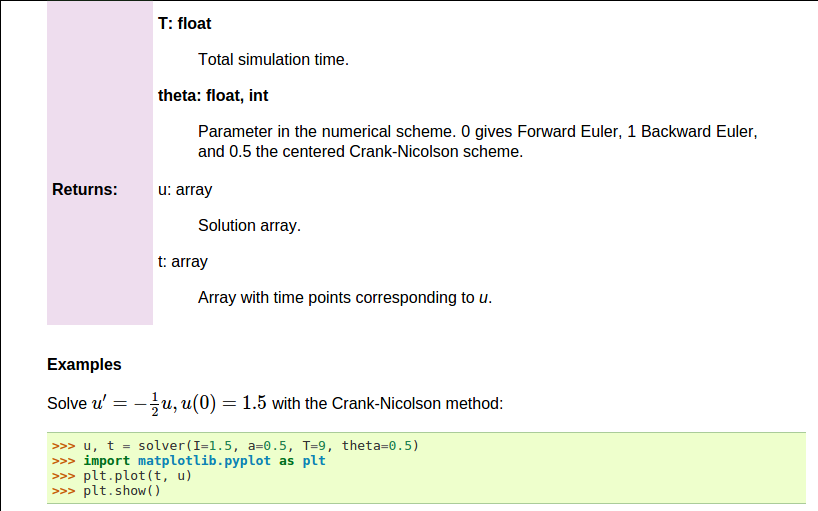
\includegraphics[width=0.8\linewidth]{fig-softeng/selfdoc_numpy.png}}
  \caption{
  Example on Sphinx API manual in HTML. \label{softeng1:basic:docstring:fig}
  }
\end{figure}
%\clearpage % flush figures softeng1:basic:docstring:fig


\subsection{Logging intermediate results}
\label{softeng1:basic:logging}

\index{logging@{\rm\texttt{logging}} module}
\index{logger}
\index{debugging}

Sometimes one may wish that a simulation program could write out
intermediate results for inspection. This could be accomplished by
a (global) \texttt{verbose} variable and code like

\begin{cod}{cbg_blue1}\begin{Verbatim}[numbers=none,fontsize=\fontsize{9pt}{9pt},baselinestretch=0.95,xleftmargin=2mm]
if verbose >= 2:
    print 'u[%d]=%g' % (i, u[i])
\end{Verbatim}
\end{cod}
\noindent
The professional way to do report intermediate results and problems is,
however, to use a \emph{logger}. This is an object that writes messages
to a log file. The messages are classified as debug, info, and warning.

\paragraph{Introductory example.}
Here is a simple example using defining a logger, using Python's \texttt{logging}
module:

\begin{pro}{cbg_blue1}{bar_blue1}\begin{Verbatim}[numbers=none,fontsize=\fontsize{9pt}{9pt},baselinestretch=0.95,xleftmargin=2mm]
import logging
logging.basicConfig(
    filename='myprog.log', filemode='w', level=logging.WARNING,
    format='%(asctime)s - %(levelname)s - %(message)s',
    datefmt='%m/%d/%Y %I:%M:%S %p')
logging.info('Here is some general info.')
logging.warning('Here is a warning.')
logging.debug('Here is some debugging info.')
logging.critical('Dividing by zero!')
logging.error('Encountered an error.')
\end{Verbatim}
\end{pro}
\noindent
Running this program gives the following output in the log file \texttt{myprog.log}:

\begin{cod}{cbg_blue1}\begin{Verbatim}[numbers=none,fontsize=\fontsize{9pt}{9pt},baselinestretch=0.95,xleftmargin=2mm]
09/26/2015 09:25:10 AM - INFO - Here is some general info.
09/26/2015 09:25:10 AM - WARNING - Here is a warning.
09/26/2015 09:25:10 AM - CRITICAL - Dividing by zero!
09/26/2015 09:25:10 AM - ERROR - Encountered an error.
\end{Verbatim}
\end{cod}
\noindent
The logger has different \emph{levels} of messages, ordered as
\emph{critical}, \emph{error}, \emph{warning}, \emph{info}, and \emph{debug}.
The \texttt{level} argument to \texttt{logging.basicConfig} sets the level
and thereby determines what the logger will print to the file:
all messages at the specified \emph{and lower} levels are printed.
For example, in the above example we set the level to be
\emph{info}, and therefore the critical, error, warning, and info
messages were printed, but not the debug message.
Setting level to debug (\texttt{logging.DEBUG}) prints all messages,
while level \emph{critical} prints only the critical messages.

The \texttt{filemode} argument is set to \texttt{w} such that any existing
log file is overwritten (the default is \texttt{a}, which means append
new messages to an existing log file, but this is seldom what
you want in mathematical computations).

The messages are preceded by the date and time and the level of
the message. This output is governed by the \texttt{format} argument:
\texttt{asctime} is the date and time, \texttt{levelname} is the name of
the message level, and \texttt{message} is the message itself.
Setting \Verb!format='%(message)s'! ensures that just the message and
nothing more is printed on each line. The \texttt{datefmt} string
specifies the formatting of the date and time, using the
rules of the \href{{https://docs.python.org/2/library/time.html#time.strftime}}{\nolinkurl{time.strftime}} function.

\paragraph{Using a logger in our solver function.}
Let us let a logger write out intermediate results and some debugging
results in the \texttt{solver} function. Such messages are useful for
monitoring the simulation and for debugging it, respectively.

\begin{cod}{cbg_blue1}\begin{Verbatim}[numbers=none,fontsize=\fontsize{9pt}{9pt},baselinestretch=0.95,xleftmargin=2mm]
import logging
logging.basicConfig(
    filename='decay.log', filemode='w', level=logging.DEBUG,
    format='%(asctime)s - %(levelname)s - %(message)s',
    datefmt='%Y.%m.%d %I:%M:%S %p')

def solver_with_logging(I, a, T, dt, theta):
    """Solve u'=-a*u, u(0)=I, for t in (0,T] with steps of dt."""
    dt = float(dt)               # avoid integer division
    Nt = int(round(T/dt))        # no of time intervals
    T = Nt*dt                    # adjust T to fit time step dt
    u = np.zeros(Nt+1)           # array of u[n] values
    t = np.linspace(0, T, Nt+1)  # time mesh
    logging.debug('solver: dt=%g, Nt=%g, T=%g' % (dt, Nt, T))

    u[0] = I                  # assign initial condition
    for n in range(0, Nt):    # n=0,1,...,Nt-1
        u[n+1] = (1 - (1-theta)*a*dt)/(1 + theta*dt*a)*u[n]

        logging.info('u[%d]=%g' % (n, u[n]))
        logging.debug('1 - (1-theta)*a*dt: %g, %s' %
                      (1-(1-theta)*a*dt,
                       str(type(1-(1-theta)*a*dt))[7:-2]))
        logging.debug('1 + theta*dt*a: %g, %s' %
                      (1 + theta*dt*a,
                       str(type(1 + theta*dt*a))[7:-2]))
    return u, t
\end{Verbatim}
\end{cod}
\noindent
We can run this new solver function in a shell:

\begin{cod}{cbg_blue1}\begin{Verbatim}[numbers=none,fontsize=\fontsize{9pt}{9pt},baselinestretch=0.95,xleftmargin=2mm]
>>> import decay
>>> u, t = decay.solver_with_logging(I=1, a=0.5, T=10, \ 
           dt=0.5, theta=0.5)
\end{Verbatim}
\end{cod}
\noindent
During this execution, each logging message is appended to the log file.
Suppose we add some pause (\texttt{time.sleep(2)}) at each time level such that
the execution takes some time. In another terminal window we can then
monitor the evolution of \texttt{decay.log} and the simulation
by the \texttt{tail -f} Unix command:

\begin{cod}{cbg_blue1}\begin{Verbatim}[numbers=none,fontsize=\fontsize{9pt}{9pt},baselinestretch=0.95,xleftmargin=2mm]
Terminal> tail -f decay.log
2015.09.26 05:37:41 AM - INFO - u[0]=1
2015.09.26 05:37:41 AM - INFO - u[1]=0.777778
2015.09.26 05:37:41 AM - INFO - u[2]=0.604938
2015.09.26 05:37:41 AM - INFO - u[3]=0.470508
2015.09.26 05:37:41 AM - INFO - u[4]=0.36595
2015.09.26 05:37:41 AM - INFO - u[5]=0.284628
\end{Verbatim}
\end{cod}
\noindent
Especially in simulation where each time step demands considerable
CPU time (minutes, hours), it can be handy to monitor such a log file
to see the evolution of the simulation.

If we want to look more closely into the numerator and denominator of
the formula for $u^{n+1}$, we can change the logging level to
\texttt{level=logging.DEBUG} and get output in \texttt{decay.log} like

\begin{cod}{cbg_blue1}\begin{Verbatim}[numbers=none,fontsize=\fontsize{9pt}{9pt},baselinestretch=0.95,xleftmargin=2mm]
2015.09.26 05:40:01 AM - DEBUG - solver: dt=0.5, Nt=20, T=10
2015.09.26 05:40:01 AM - INFO - u[0]=1
2015.09.26 05:40:01 AM - DEBUG - 1 - (1-theta)*a*dt: 0.875, float
2015.09.26 05:40:01 AM - DEBUG - 1 + theta*dt*a: 1.125, float
2015.09.26 05:40:01 AM - INFO - u[1]=0.777778
2015.09.26 05:40:01 AM - DEBUG - 1 - (1-theta)*a*dt: 0.875, float
2015.09.26 05:40:01 AM - DEBUG - 1 + theta*dt*a: 1.125, float
2015.09.26 05:40:01 AM - INFO - u[2]=0.604938
2015.09.26 05:40:01 AM - DEBUG - 1 - (1-theta)*a*dt: 0.875, float
2015.09.26 05:40:01 AM - DEBUG - 1 + theta*dt*a: 1.125, float
2015.09.26 05:40:01 AM - INFO - u[3]=0.470508
2015.09.26 05:40:01 AM - DEBUG - 1 - (1-theta)*a*dt: 0.875, float
2015.09.26 05:40:01 AM - DEBUG - 1 + theta*dt*a: 1.125, float
2015.09.26 05:40:01 AM - INFO - u[4]=0.36595
2015.09.26 05:40:01 AM - DEBUG - 1 - (1-theta)*a*dt: 0.875, float
2015.09.26 05:40:01 AM - DEBUG - 1 + theta*dt*a: 1.125, float
\end{Verbatim}
\end{cod}
\noindent


\section{User interfaces}
\label{softeng1:basic:UI}

It is good programming practice to let programs read input from
some \emph{user interface}, rather than requiring users to \emph{edit}
parameter values in the source code. With effective user interfaces
it becomes easier and safer to apply the code for scientific investigations and
in particular to automate large-scale investigations by other programs
(see Section~\ref{softeng1:experiments}).

Reading input data can be done in many ways. We have to decide on the
functionality of the user interface, i.e., how we want to operate the
program when providing input. Thereafter, we use appropriate tools to
implement the particular user interface. There are four basic types
of user interface, listed here according to implementational
complexity, from lowest to highest:

\begin{enumerate}
\item Questions and answers in the terminal window

\item Command-line arguments

\item Reading data from files

\item Graphical user interfaces (GUIs)
\end{enumerate}

\noindent
Personal preferences of user interfaces differ substantially, and it is
difficult to present recommendations or pros and cons.
Alternatives 2 and 4 are most popular and will be addressed next.
The goal is to make it easy for the user to
set physical and numerical parameters in
our \texttt{decay.py} program. However, we use  a little toy program, called
\texttt{prog.py}, as introductory
example:

\begin{pro}{cbg_blue1}{bar_blue1}\begin{Verbatim}[numbers=none,fontsize=\fontsize{9pt}{9pt},baselinestretch=0.95,xleftmargin=2mm]
delta = 0.5
p = 2
from math import exp
result = delta*exp(-p)
print result
\end{Verbatim}
\end{pro}
\noindent
The essential content is that \texttt{prog.py} has two input parameters: \texttt{delta}
and \texttt{p}. A user interface will replace the first two assignments to
\texttt{delta} and \texttt{p}.

\subsection{Command-line arguments}

The command-line arguments are all the words that appear on the
command line after the program name. Running a program \texttt{prog.py}
as \texttt{python prog.py arg1 arg2} means that there are two command-line arguments
(separated by white space): \texttt{arg1} and \texttt{arg2}.
Python stores all command-line arguments in
a special list \texttt{sys.argv}. (The name \texttt{argv} stems from the C language and
stands for ``argument values''. In C there is also an integer variable
called \texttt{argc} reflecting the number of arguments, or ``argument counter''.
A lot of programming languages have adopted the variable name \texttt{argv} for
the command-line arguments.)
Here is an example on a
program \Verb!what_is_sys_argv.py! that can show us what the command-line arguments
are

\begin{pro}{cbg_blue1}{bar_blue1}\begin{Verbatim}[numbers=none,fontsize=\fontsize{9pt}{9pt},baselinestretch=0.95,xleftmargin=2mm]
import sys
print sys.argv
\end{Verbatim}
\end{pro}
\noindent
A sample run goes like

\begin{Verbatim}[frame=lines,label=\fbox{{\tiny Terminal}},framesep=2.5mm,framerule=0.7pt,fontsize=\fontsize{9pt}{9pt}]
Terminal> python what_is_sys_argv.py 5.0 'two words' -1E+4
['what_is_sys_argv.py', '5.0', 'two words', '-1E+4']
\end{Verbatim}
We make two observations:

\begin{itemize}
 \item \texttt{sys.argv[0]} is the name of the program,
   and the sublist \texttt{sys.argv[1:]} contains all the command-line arguments.

 \item Each command-line argument is available as a string. A conversion to
   \texttt{float} is necessary if we want to compute with the numbers 5.0 and
   $10^4$.
\end{itemize}

\noindent
There are, in principle, two ways of programming with
command-line arguments in Python:

\begin{itemize}
 \item \textbf{Positional arguments:} Decide upon a sequence of parameters
   on the command line and read
   their values directly from the \texttt{sys.argv[1:]} list.

 \item \textbf{Option-value pairs:}  Use \texttt{--option value} on
   the command line to replace the default value of an input parameter
   \texttt{option} by \texttt{value} (and utilize the \texttt{argparse.ArgumentParser} tool
   for implementation).
\end{itemize}

\noindent
Suppose we want to run some program \texttt{prog.py} with
specification of two parameters \texttt{p} and \texttt{delta} on the command line.
With positional command-line arguments we write

\begin{Verbatim}[frame=lines,label=\fbox{{\tiny Terminal}},framesep=2.5mm,framerule=0.7pt,fontsize=\fontsize{9pt}{9pt}]
Terminal> python prog.py 2 0.5
\end{Verbatim}
and must know that the first argument \texttt{2} represents \texttt{p} and the
next \texttt{0.5} is the value of \texttt{delta}.
With option-value pairs we can run

\begin{Verbatim}[frame=lines,label=\fbox{{\tiny Terminal}},framesep=2.5mm,framerule=0.7pt,fontsize=\fontsize{9pt}{9pt}]
Terminal> python prog.py --delta 0.5 --p 2
\end{Verbatim}
Now, both \texttt{p} and \texttt{delta} are supposed to have default values in the program,
so we need to specify only the parameter that is to be changed from
its default value, e.g.,

\begin{Verbatim}[frame=lines,label=\fbox{{\tiny Terminal}},framesep=2.5mm,framerule=0.7pt,fontsize=\fontsize{9pt}{9pt}]
Terminal> python prog.py --p 2         # p=2, default delta
Terminal> python prog.py --delta 0.7   # delta-0.7, default a
Terminal> python prog.py               # default a and delta
\end{Verbatim}

How do we extend the \texttt{prog.py} code for positional arguments
and option-value pairs? Positional arguments require very simple
code:

\begin{pro}{cbg_blue1}{bar_blue1}\begin{Verbatim}[numbers=none,fontsize=\fontsize{9pt}{9pt},baselinestretch=0.95,xleftmargin=2mm]
import sys
p = float(sys.argv[1])
delta = float(sys.argv[2])

from math import exp
result = delta*exp(-p)
print result
\end{Verbatim}
\end{pro}
\noindent
If the user forgets to supply two command-line arguments, Python will
raise an \texttt{IndexError} exception and produce a long error message.
To avoid that, we should use a \texttt{try-except} construction:

\begin{pro}{cbg_blue1}{bar_blue1}\begin{Verbatim}[numbers=none,fontsize=\fontsize{9pt}{9pt},baselinestretch=0.95,xleftmargin=2mm]
import sys
try:
    p = float(sys.argv[1])
    delta = float(sys.argv[2])
except IndexError:
    print 'Usage: %s p delta' % sys.argv[0]
    sys.exit(1)

from math import exp
result = delta*exp(-p)
print result
\end{Verbatim}
\end{pro}
\noindent
Using \texttt{sys.exit(1)} aborts the program. The value 1 (actually any
value different from 0) notifies the operating system that the
program failed.


\begin{warning_mdfboxadmon}[Command-line arguments are strings!]
Note that all elements in \texttt{sys.argv} are string objects.
If the values are used in mathematical computations, we need
to explicitly convert the strings to numbers.
\end{warning_mdfboxadmon}



Option-value pairs requires more programming and is actually
better explained in a more comprehensive example below.
Minimal code for our \texttt{prog.py} program reads

\begin{pro}{cbg_blue1}{bar_blue1}\begin{Verbatim}[numbers=none,fontsize=\fontsize{9pt}{9pt},baselinestretch=0.95,xleftmargin=2mm]
import argparse
parser = argparse.ArgumentParser()
parser.add_argument('--p', default=1.0)
parser.add_argument('--delta', default=0.1)

args = parser.parse_args()
p = args.p
delta = args.delta

from math import exp
result = delta*exp(-p)
print result
\end{Verbatim}
\end{pro}
\noindent
Because the default values of \texttt{delta} and \texttt{p} are float numbers,
the \texttt{args.delta} and \texttt{args.p} variables are automatically of type \texttt{float}.

Our next task is to use these basic code constructs to equip our
\texttt{decay.py} module with command-line interfaces.

\subsection{Positional command-line arguments}

\index{list comprehension}
\index{sys.argv@{\rm\texttt{sys.argv}}}
\index{command-line arguments}

For our \texttt{decay.py} module file, we want to include functionality such
that we can read $I$, $a$, $T$, $\theta$, and a range of $\Delta t$
values from the command line.  A plot is then to be made, comparing
the different numerical solutions for different $\Delta t$ values
against the exact solution. The technical details of getting the
command-line information into the program is covered in the next
two sections.

The simplest way of reading the input parameters is to
decide on their sequence on the command line and just index
the \texttt{sys.argv} list accordingly.
Say the sequence of input data for some functionality in
\texttt{decay.py} is $I$, $a$, $T$, $\theta$ followed by an
arbitrary number of $\Delta t$ values. This code extracts
these \emph{positional} command-line arguments:

\begin{cod}{cbg_blue1}\begin{Verbatim}[numbers=none,fontsize=\fontsize{9pt}{9pt},baselinestretch=0.95,xleftmargin=2mm]
def read_command_line_positional():
    if len(sys.argv) < 6:
        print 'Usage: %s I a T on/off BE/FE/CN dt1 dt2 dt3 ...' % \ 
              sys.argv[0]; sys.exit(1)  # abort

    I = float(sys.argv[1])
    a = float(sys.argv[2])
    T = float(sys.argv[3])
    theta = float(sys.argv[4])
    dt_values = [float(arg) for arg in sys.argv[5:]]

    return I, a, T, theta, dt_values
\end{Verbatim}
\end{cod}
\noindent
Note that we may use a \texttt{try-except} construction instead of the if test.

A run like

\begin{Verbatim}[frame=lines,label=\fbox{{\tiny Terminal}},framesep=2.5mm,framerule=0.7pt,fontsize=\fontsize{9pt}{9pt}]
Terminal> python decay.py 1 0.5 4 0.5 1.5 0.75 0.1
\end{Verbatim}
results in

\begin{cod}{cbg_blue1}\begin{Verbatim}[numbers=none,fontsize=\fontsize{9pt}{9pt},baselinestretch=0.95,xleftmargin=2mm]
sys.argv = ['decay.py', '1', '0.5', '4', '0.5', '1.5', '0.75', '0.1']
\end{Verbatim}
\end{cod}
\noindent
and consequently the assignments \texttt{I=1.0}, \texttt{a=0.5}, \texttt{T=4.0}, \texttt{thet=0.5},
and \Verb!dt_values = [1.5, 0.75, 0.1]!.

Instead of specifying the $\theta$ value, we could be a bit more
sophisticated and let the user write the name of the scheme:
\texttt{BE} for Backward Euler, \texttt{FE} for Forward Euler, and \texttt{CN}
for Crank-Nicolson. Then we must map this string to the proper
$\theta$ value, an operation elegantly done by a dictionary:

\begin{cod}{cbg_blue1}\begin{Verbatim}[numbers=none,fontsize=\fontsize{9pt}{9pt},baselinestretch=0.95,xleftmargin=2mm]
scheme = sys.argv[4]
scheme2theta = {'BE': 1, 'CN': 0.5, 'FE': 0}
if scheme in scheme2theta:
    theta = scheme2theta[scheme]
else:
    print 'Invalid scheme name:', scheme; sys.exit(1)
\end{Verbatim}
\end{cod}
\noindent
Now we can do

\begin{Verbatim}[frame=lines,label=\fbox{{\tiny Terminal}},framesep=2.5mm,framerule=0.7pt,fontsize=\fontsize{9pt}{9pt}]
Terminal> python decay.py 1 0.5 4 CN 1.5 0.75 0.1
\end{Verbatim}
and get `theta=0.5`in the code.


\subsection{Option-value pairs on the command line}

\index{argparse@{\rm\texttt{argparse}} (Python module)}
\index{ArgumentParser@{\rm\texttt{ArgumentParser}} (Python class)}
\index{option-value pairs (command line)}
\index{command-line arguments}
\index{reading the command line}

Now we want to specify option-value pairs on the command line,
using \texttt{--I} for \texttt{I} ($I$), \texttt{--a} for \texttt{a} ($a$), \texttt{--T} for \texttt{T} ($T$),
\texttt{--scheme} for the scheme name (\texttt{BE}, \texttt{FE}, \texttt{CN}),
and \texttt{--dt} for the sequence of \texttt{dt} ($\Delta t$) values.
Each parameter must have a sensible default value so
that we specify the option on the command line only when the default
value is not suitable. Here is a typical run:

\begin{Verbatim}[frame=lines,label=\fbox{{\tiny Terminal}},framesep=2.5mm,framerule=0.7pt,fontsize=\fontsize{9pt}{9pt}]
Terminal> python decay.py --I 2.5 --dt 0.1 0.2 0.01 --a 0.4
\end{Verbatim}
Observe the major advantage over positional command-line arguments:
the input is much easier to read and much easier to write.
With positional arguments it is easy to mess up the sequence of
the input parameters and quite challenging to detect errors too,
unless there are just a couple of arguments.

Python's \texttt{ArgumentParser} tool in the \texttt{argparse} module makes it easy
to create a professional command-line interface to any program. The
documentation of \href{{http://docs.python.org/library/argparse.html}}{\nolinkurl{ArgumentParser}} demonstrates its
versatile applications, so we shall here just list an example
containing the most basic features. It always pays off to use \texttt{ArgumentParser}
rather than trying to manually inspect and interpret option-value pairs
in \texttt{sys.argv}!

The use of \texttt{ArgumentParser} typically involves three steps:

\begin{cod}{cbg_blue1}\begin{Verbatim}[numbers=none,fontsize=\fontsize{9pt}{9pt},baselinestretch=0.95,xleftmargin=2mm]
import argparse
parser = argparse.ArgumentParser()

# Step 1: add arguments
parser.add_argument('--option_name', ...)

# Step 2: interpret the command line
args = parser.parse_args()

# Step 3: extract values
value = args.option_name
\end{Verbatim}
\end{cod}
\noindent

A function for setting up all the options is handy:

\begin{cod}{cbg_blue1}\begin{Verbatim}[numbers=none,fontsize=\fontsize{9pt}{9pt},baselinestretch=0.95,xleftmargin=2mm]
def define_command_line_options():
    import argparse
    parser = argparse.ArgumentParser()
    parser.add_argument(
        '--I', '--initial_condition', type=float,
        default=1.0, help='initial condition, u(0)',
        metavar='I')
    parser.add_argument(
        '--a', type=float, default=1.0,
        help='coefficient in ODE', metavar='a')
    parser.add_argument(
        '--T', '--stop_time', type=float,
        default=1.0, help='end time of simulation',
        metavar='T')
    parser.add_argument(
        '--scheme', type=str, default='CN',
        help='FE, BE, or CN')
    parser.add_argument(
        '--dt', '--time_step_values', type=float,
        default=[1.0], help='time step values',
        metavar='dt', nargs='+', dest='dt_values')
    return parser
\end{Verbatim}
\end{cod}
\noindent

Each command-line option is defined through the \Verb!parser.add_argument!
method\footnote{We use the expression \emph{method} here, because \texttt{parser} is a class variable and functions in classes are known as methods in Python and many other languages. Readers not familiar with class programming can just substitute this use of \emph{method} by \emph{function}.}. Alternative options, like the short \texttt{--I} and the more
explaining version \Verb!--initial_condition! can be defined. Other arguments
are \texttt{type} for the Python object type, a default value, and a help
string, which gets printed if the command-line argument \texttt{-h} or \texttt{--help} is
included. The \texttt{metavar} argument specifies the value associated with
the option when the help string is printed. For example, the option for
$I$ has this help output:

\begin{Verbatim}[frame=lines,label=\fbox{{\tiny Terminal}},framesep=2.5mm,framerule=0.7pt,fontsize=\fontsize{9pt}{9pt}]
Terminal> python decay.py -h
  ...
  --I I, --initial_condition I
                        initial condition, u(0)
  ...
\end{Verbatim}
The structure of this output is

\begin{cod}{cbg_blue1}\begin{Verbatim}[numbers=none,fontsize=\fontsize{9pt}{9pt},baselinestretch=0.95,xleftmargin=2mm]
  --I metavar, --initial_condition metavar
                        help-string
\end{Verbatim}
\end{cod}
\noindent



Finally, the \texttt{--dt} option demonstrates how to allow for more than one
value (separated by blanks) through the \texttt{nargs='+'} keyword argument.
After the command line is parsed, we get an object where the values of
the options are stored as attributes. The attribute name is specified
by the \texttt{dist} keyword argument, which for the \texttt{--dt} option is
\Verb!dt_values!. Without the \texttt{dest} argument, the value of an option \texttt{--opt}
is stored as the attribute \texttt{opt}.

The code below demonstrates how to read the command line and extract
the values for each option:

\begin{cod}{cbg_blue1}\begin{Verbatim}[numbers=none,fontsize=\fontsize{9pt}{9pt},baselinestretch=0.95,xleftmargin=2mm]
def read_command_line_argparse():
    parser = define_command_line_options()
    args = parser.parse_args()
    scheme2theta = {'BE': 1, 'CN': 0.5, 'FE': 0}
    data = (args.I, args.a, args.T, scheme2theta[args.scheme],
            args.dt_values)
    return data
\end{Verbatim}
\end{cod}
\noindent
As seen, the values of the command-line options are available as
attributes in \texttt{args}: \texttt{args.opt} holds the value of option \texttt{--opt}, unless
we used the \texttt{dest} argument (as for \Verb!--dt_values!) for specifying the
attribute name. The \texttt{args.opt} attribute has the object type specified
by \texttt{type} (\texttt{str} by default).

The making of the plot is not dependent on whether we read data from
the command line as positional arguments or option-value pairs:

\begin{cod}{cbg_blue1}\begin{Verbatim}[numbers=none,fontsize=\fontsize{9pt}{9pt},baselinestretch=0.95,xleftmargin=2mm]
def experiment_compare_dt(option_value_pairs=False):
    I, a, T, theta, dt_values = \ 
       read_command_line_argparse() if option_value_pairs else \ 
       read_command_line_positional()

    legends = []
    for dt in dt_values:
        u, t = solver(I, a, T, dt, theta)
        plt.plot(t, u)
        legends.append('dt=%g' % dt)
    t_e = np.linspace(0, T, 1001)       # very fine mesh for u_e
    u_e = u_exact(t_e, I, a)
    plt.plot(t_e, u_e, '--')
    legends.append('exact')
    plt.legend(legends, loc='upper right')
    plt.title('theta=%g' % theta)
    plotfile = 'tmp'
    plt.savefig(plotfile + '.png');  plt.savefig(plotfile + '.pdf')
\end{Verbatim}
\end{cod}
\noindent


\subsection{Creating a graphical web user interface}

The Python package \href{{https://github.com/hplgit/parampool}}{Parampool}
can be used to automatically generate a web-based \emph{graphical user interface}
(GUI) for our simulation program. Although the programming technique
dramatically simplifies the efforts to create a GUI, the forthcoming
material on equipping our \texttt{decay} module with a GUI is quite technical
and of significantly less importance than knowing how to make
a command-line interface.

\paragraph{Making a compute function.}
The first step is to identify a function
that performs the computations and that takes the necessary input
variables as arguments. This is called the \emph{compute function} in
Parampool terminology. The purpose of this function is to take
values of $I$, $a$, $T$ together with a sequence of $\Delta t$ values
and a sequence of $\theta$ and plot the numerical against the
exact solution for each pair of $(\theta, \Delta t)$.
The plots can be arranged as a table with the columns being scheme type
($\theta$ value) and the rows reflecting the discretization parameter
($\Delta t$ value). Figure~\ref{softeng1:fig:GUI} displays what the
graphical web interface may look like after results are computed
(there are $3\times 3$ plots in the GUI, but only $2\times 2$ are
visible in the figure).


\begin{figure}[!ht]  % softeng1:fig:GUI
  \centerline{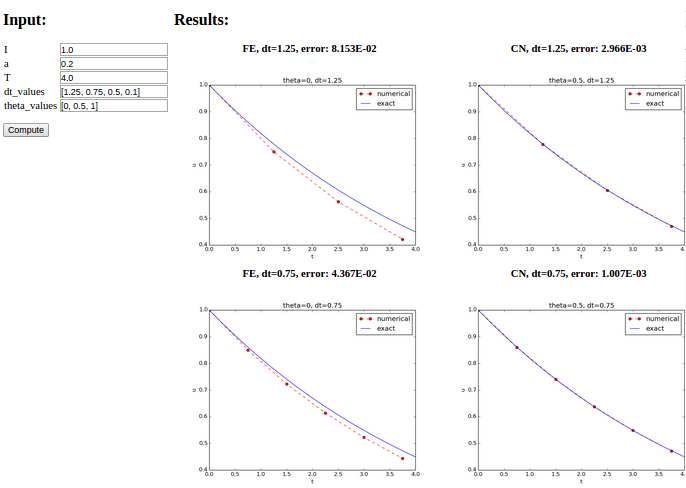
\includegraphics[width=1.0\linewidth]{fig-softeng/web_GUI.png}}
  \caption{
  Automatically generated graphical web interface. \label{softeng1:fig:GUI}
  }
\end{figure}
%\clearpage % flush figures softeng1:fig:GUI



To tell Parampool what type of input data we have,
we assign default values of the right type to all arguments in the
compute function, here called \Verb!main_GUI!:

\begin{cod}{cbg_blue1}\begin{Verbatim}[numbers=none,fontsize=\fontsize{9pt}{9pt},baselinestretch=0.95,xleftmargin=2mm]
def main_GUI(I=1.0, a=.2, T=4.0,
             dt_values=[1.25, 0.75, 0.5, 0.1],
             theta_values=[0, 0.5, 1]):
\end{Verbatim}
\end{cod}
\noindent

The compute function must return the HTML code we want for displaying
the result in a web page. Here we want to show a
table of plots.
Assume for now that the HTML code for one plot and the value of the
norm of the error can be computed by some other function \texttt{compute4web}.
The \Verb!main_GUI! function can then loop over $\Delta t$ and $\theta$
values and put each plot in an HTML table. Appropriate code goes like

\begin{cod}{cbg_blue1}\begin{Verbatim}[numbers=none,fontsize=\fontsize{9pt}{9pt},baselinestretch=0.95,xleftmargin=2mm]
def main_GUI(I=1.0, a=.2, T=4.0,
             dt_values=[1.25, 0.75, 0.5, 0.1],
             theta_values=[0, 0.5, 1]):
    # Build HTML code for web page. Arrange plots in columns
    # corresponding to the theta values, with dt down the rows
    theta2name = {0: 'FE', 1: 'BE', 0.5: 'CN'}
    html_text = '<table>\n'
    for dt in dt_values:
        html_text += '<tr>\n'
        for theta in theta_values:
            E, html = compute4web(I, a, T, dt, theta)
            html_text += """
<td>
<center><b>%s, dt=%g, error: %.3E</b></center><br>
%s
</td>
""" % (theta2name[theta], dt, E, html)
        html_text += '</tr>\n'
    html_text += '</table>\n'
    return html_text
\end{Verbatim}
\end{cod}
\noindent

Making one plot is done in \texttt{compute4web}. The statements should be
straightforward from earlier examples, but there is one new feature:
we use a tool in Parampool to embed the PNG code for a plot file
directly in an HTML image tag. The details are hidden from the
programmer, who can just rely on
relevant HTML code in the string \Verb!html_text!. The function looks like

\begin{cod}{cbg_blue1}\begin{Verbatim}[numbers=none,fontsize=\fontsize{9pt}{9pt},baselinestretch=0.95,xleftmargin=2mm]
def compute4web(I, a, T, dt, theta=0.5):
    """
    Run a case with the solver, compute error measure,
    and plot the numerical and exact solutions in a PNG
    plot whose data are embedded in an HTML image tag.
    """
    u, t = solver(I, a, T, dt, theta)
    u_e = u_exact(t, I, a)
    e = u_e - u
    E = np.sqrt(dt*np.sum(e**2))

    plt.figure()
    t_e = np.linspace(0, T, 1001)    # fine mesh for u_e
    u_e = u_exact(t_e, I, a)
    plt.plot(t,   u,   'r--o')
    plt.plot(t_e, u_e, 'b-')
    plt.legend(['numerical', 'exact'])
    plt.xlabel('t')
    plt.ylabel('u')
    plt.title('theta=%g, dt=%g' % (theta, dt))
    # Save plot to HTML img tag with PNG code as embedded data
    from parampool.utils import save_png_to_str
    html_text = save_png_to_str(plt, plotwidth=400)

    return E, html_text
\end{Verbatim}
\end{cod}
\noindent


\paragraph{Generating the user interface.}
The web GUI is automatically generated by
the following code, placed in the file \href{{http://tinyurl.com/ofkw6kc/softeng/decay_GUI_generate.py}}{\nolinkurl{decay_GUI_generate.py}}.

\begin{pro}{cbg_blue1}{bar_blue1}\begin{Verbatim}[numbers=none,fontsize=\fontsize{9pt}{9pt},baselinestretch=0.95,xleftmargin=2mm]
from parampool.generator.flask import generate
from decay import main_GUI
generate(main_GUI,
         filename_controller='decay_GUI_controller.py',
         filename_template='decay_GUI_view.py',
         filename_model='decay_GUI_model.py')
\end{Verbatim}
\end{pro}
\noindent
Running the \Verb!decay_GUI_generate.py! program results in three new
files whose names are specified in the call to \texttt{generate}:

\begin{enumerate}
 \item \Verb!decay_GUI_model.py! defines HTML widgets to be used to set
    input data in the web interface,

 \item \Verb!templates/decay_GUI_views.py! defines the layout of the web page,

 \item \Verb!decay_GUI_controller.py! runs the web application.
\end{enumerate}

\noindent
We only need to run the last program, and there is no need to look into
these files.

\paragraph{Running the web application.}
The web GUI is started by

\begin{Verbatim}[frame=lines,label=\fbox{{\tiny Terminal}},framesep=2.5mm,framerule=0.7pt,fontsize=\fontsize{9pt}{9pt}]
Terminal> python decay_GUI_controller.py
\end{Verbatim}
Open a web browser at the location \texttt{127.0.0.1:5000}. Input fields for
\texttt{I}, \texttt{a}, \texttt{T}, \Verb!dt_values!, and \Verb!theta_values! are presented.  Figure~\ref{softeng1:fig:GUI} shows a part of the resulting page if we run
with the default values for the input parameters.
With the techniques demonstrated here, one can
easily create a tailored web GUI for a particular type of application
and use it to interactively explore physical and numerical effects.

\section{Tests for verifying implementations}

Any module with functions should have a set of tests that can
check the
correctness of the implementations.
There exists
well-established procedures and corresponding tools for automating
the execution of such tests. These tools allow large test sets to be
run with a one-line command, making it easy to check that the
software still works (as far as the
tests can tell!). Here we shall illustrate two important
software testing techniques: \emph{doctest} and \emph{unit testing}.
The first one is Python specific, while unit testing is the dominating
test technique in the software industry today.

\subsection{Doctests}

\index{doctests}
\index{software testing!doctests}

A doc string, the first string after the function header, is used to
document the purpose of functions and their arguments
(see Section~\ref{softeng1:basic:func}). Very often it
is instructive to include an example in the doc string
on how to use the function.
Interactive examples in the Python shell are most illustrative as
we can see the output resulting from the statements and expressions.
For example,
in the \texttt{solver} function, we can include an example on calling
this function and printing the computed \texttt{u} and \texttt{t} arrays:

\begin{cod}{cbg_blue1}\begin{Verbatim}[numbers=none,fontsize=\fontsize{9pt}{9pt},baselinestretch=0.95,xleftmargin=2mm]
def solver(I, a, T, dt, theta):
    """
    Solve u'=-a*u, u(0)=I, for t in (0,T] with steps of dt.


    >>> u, t = solver(I=0.8, a=1.2, T=1.5, dt=0.5, theta=0.5)
    >>> for n in range(len(t)):
    ...     print 't=%.1f, u=%.14f' % (t[n], u[n])
    t=0.0, u=0.80000000000000
    t=0.5, u=0.43076923076923
    t=1.0, u=0.23195266272189
    t=1.5, u=0.12489758761948
    """
    ...
\end{Verbatim}
\end{cod}
\noindent

When such interactive demonstrations are inserted in doc strings,
Python's \href{{http://docs.python.org/library/doctest.html}}{\nolinkurl{doctest}}
module can be used to automate running all commands
in interactive sessions and compare new output with the output
appearing in the doc string.  All we have to do in the current example
is to run the module file \texttt{decay.py} with

\begin{cod}{cbg_blue1}\begin{Verbatim}[numbers=none,fontsize=\fontsize{9pt}{9pt},baselinestretch=0.95,xleftmargin=2mm]
Terminal> python -m doctest decay.py
\end{Verbatim}
\end{cod}
\noindent
This command imports the \texttt{doctest} module, which runs all
doctests found in the file and reports discrepancies between
expected and computed output.
Alternatively, the test block in a module may run all doctests
by

\begin{cod}{cbg_blue1}\begin{Verbatim}[numbers=none,fontsize=\fontsize{9pt}{9pt},baselinestretch=0.95,xleftmargin=2mm]
if __name__ == '__main__':
    import doctest
    doctest.testmod()
\end{Verbatim}
\end{cod}
\noindent
Doctests can also be embedded in nose/pytest unit tests
as explained in the next section.


\begin{warning_mdfboxadmon}[Doctests prevent command-line arguments!]
No additional command-line argument is allowed when running doctests.
If your program relies on command-line input, make sure the doctests
can be run \emph{without} such input on the command line.

However, you can simulate command-line input by filling \texttt{sys.argv}
with values, e.g.,

\begin{cod}{cbg_blue1}\begin{Verbatim}[numbers=none,fontsize=\fontsize{9pt}{9pt},baselinestretch=0.95,xleftmargin=2mm]
import sys; sys.argv = '--I 1.0 --a 5'.split()
\end{Verbatim}
\end{cod}
\noindent
\end{warning_mdfboxadmon}



The execution command above will report any problem if a test fails.
As an illustration, let us alter the \texttt{u} value at \texttt{t=1.5} in
the output of the doctest by replacing the last digit \texttt{8} by \texttt{7}.
This edit triggers a report:

\begin{Verbatim}[frame=lines,label=\fbox{{\tiny Terminal}},framesep=2.5mm,framerule=0.7pt,fontsize=\fontsize{9pt}{9pt}]
Terminal> python -m doctest decay.py
********************************************************
File "decay.py", line ...
Failed example:
    for n in range(len(t)):
        print 't=%.1f, u=%.14f' % (t[n], u[n])
Expected:
    t=0.0, u=0.80000000000000
    t=0.5, u=0.43076923076923
    t=1.0, u=0.23195266272189
    t=1.5, u=0.12489758761948
Got:
    t=0.0, u=0.80000000000000
    t=0.5, u=0.43076923076923
    t=1.0, u=0.23195266272189
    t=1.5, u=0.12489758761947
\end{Verbatim}


\begin{warning_mdfboxadmon}[Pay attention to the number of digits in doctest results!]
Note that in the output of \texttt{t} and \texttt{u} we write \texttt{u} with 14 digits.
Writing all 16 digits is not a good idea: if the tests are run on
different hardware, round-off errors might be different, and
the \texttt{doctest} module detects that the numbers are not precisely the same
and reports failures. In the present application, where $0 < u(t) \leq 0.8$,
we expect round-off errors to be of size $10^{-16}$, so comparing 15
digits would probably be reliable, but we compare 14 to be on the
safe side. On the other hand, comparing a small number of digits may
hide software errors.
\end{warning_mdfboxadmon}



Doctests are highly encouraged as they do two things: 1) demonstrate
how a function is used and 2) test that the function works.


\subsection{Unit tests and test functions}

\index{nose@{\rm\texttt{nose}} tests}
\index{pytest@{\rm\texttt{pytest}} tests}
\index{unit testing}
\index{software testing!nose}
\index{software testing!pytest}

The unit testing technique consists of identifying smaller units
of code and writing one or more tests for
each unit. One unit can typically be a function.
Each test should, ideally, not depend on the outcome of
other tests. The recommended practice is actually to
design and write the unit tests first and \emph{then} implement the functions!

In scientific computing it is not always obvious how to best perform
unit testing. The units are naturally larger than in non-scientific
software. Very often the solution procedure of a mathematical problem
identifies a unit, such as our \texttt{solver} function.

\index{test function}
\index{software testing!test function}

\paragraph{Two Python test frameworks: nose and pytest.}
Python offers two very easy-to-use software frameworks for implementing
unit tests: nose and pytest. These work (almost) in the same way,
but our recommendation is to go for pytest.

\paragraph{Test function requirements.}
For a test to qualify as a \emph{test function} in nose or pytest, three
rules must be followed:

\begin{enumerate}
 \item The function name must start with \Verb!test_!.

 \item Function arguments are not allowed.

 \item An \texttt{AssertionError} exception must be raised if the test fails.
\end{enumerate}

\noindent
A specific example might be illustrative before proceeding.
We have the following function that we want to test:

\begin{cod}{cbg_blue1}\begin{Verbatim}[numbers=none,fontsize=\fontsize{9pt}{9pt},baselinestretch=0.95,xleftmargin=2mm]
def double(n):
    return 2*n
\end{Verbatim}
\end{cod}
\noindent
The corresponding test function could, in principle, have been written
as

\begin{cod}{cbg_blue1}\begin{Verbatim}[numbers=none,fontsize=\fontsize{9pt}{9pt},baselinestretch=0.95,xleftmargin=2mm]
def test_double():
    """Test that double(n) works for one specific n."""
    n = 4
    expected = 2*4
    computed = double(4)
    if expected != computed:
        raise AssertionError
\end{Verbatim}
\end{cod}
\noindent
The last two lines, however, are never written like this in test functions.
Instead, Python's \texttt{assert} statement is used: \texttt{assert success, msg}, where
\texttt{success} is a boolean variable, which is \texttt{False} if the test fails, and
\texttt{msg} is \emph{an optional} message string that is printed when the test fails.
A better version of the test function is therefore

\begin{cod}{cbg_blue1}\begin{Verbatim}[numbers=none,fontsize=\fontsize{9pt}{9pt},baselinestretch=0.95,xleftmargin=2mm]
def test_double():
    """Test that double(n) works for one specific n."""
    n = 4
    expected = 2*4
    computed = double(4)
    msg = 'expected %g, computed %g' % (expected, computed)
    success = expected == computed
    assert success, msg
\end{Verbatim}
\end{cod}
\noindent

\paragraph{Comparison of real numbers.}
Because of the finite precision arithmetics on a computer, which gives
rise to round-off errors, the \texttt{==} operator is not suitable for
checking whether two real numbers are equal. Obviously, this principle
also applies to tests in test functions.
We must therefore replace \texttt{a == b} by a comparison
based on a tolerance \texttt{tol}: \texttt{abs(a-b) < tol}. The next example illustrates
the problem and its solution.

Here is a slightly different function that
we want to test:

\begin{cod}{cbg_blue1}\begin{Verbatim}[numbers=none,fontsize=\fontsize{9pt}{9pt},baselinestretch=0.95,xleftmargin=2mm]
def third(x):
    return x/3.
\end{Verbatim}
\end{cod}
\noindent
We write a test function where the expected result is computed as
$\frac{1}{3}x$ rather than $x/3$:

\begin{cod}{cbg_blue1}\begin{Verbatim}[numbers=none,fontsize=\fontsize{9pt}{9pt},baselinestretch=0.95,xleftmargin=2mm]
def test_third():
    """Check that third(x) works for many x values."""
    for x in np.linspace(0, 1, 21):
        expected = (1/3.0)*x
        computed = third(x)
        success = expected == computed
        assert success
\end{Verbatim}
\end{cod}
\noindent
This \Verb!test_third! function executes silently, i.e., no failure,
until \texttt{x} becomes 0.15. Then round-off errors make the \texttt{==} comparison
\texttt{False}. In fact, seven of the \texttt{x} values above face this problem.
The solution is to compare \texttt{expected} and \texttt{computed}
with a small tolerance:

\begin{cod}{cbg_blue1}\begin{Verbatim}[numbers=none,fontsize=\fontsize{9pt}{9pt},baselinestretch=0.95,xleftmargin=2mm]
def test_third():
    """Check that third(x) works for many x values."""
    for x in np.linspace(0, 1, 21):
        expected = (1/3.)*x
        computed = third(x)
        tol = 1E-15
        success = abs(expected - computed) < tol
        assert success
\end{Verbatim}
\end{cod}
\noindent


\begin{notice_mdfboxadmon}[Always compare real numbers with a tolerance!]
Real numbers should never be compared with the \texttt{==} operator, but always
with the absolute value of the difference and a tolerance.
So, replace \texttt{a == b}, if \texttt{a} and/or \texttt{b} is \texttt{float}, by

\begin{cod}{cbg_blue1}\begin{Verbatim}[numbers=none,fontsize=\fontsize{9pt}{9pt},baselinestretch=0.95,xleftmargin=2mm]
tol = 1E-14
abs(a - b) < tol
\end{Verbatim}
\end{cod}
\noindent
The suitable size of \texttt{tol} depends on the size of \texttt{a} and \texttt{b}
(see Problem~\ref{softeng1:exer:tol}).
\end{notice_mdfboxadmon}



\paragraph{Special assert functions from nose.}
Test frameworks often contain more tailored
\emph{assert functions} that can be called instead of using the \texttt{assert}
statement. For example, comparing two objects within
a tolerance, as in the present
case, can be done by the \Verb!assert_almost_equal! from the nose
framework:

\begin{cod}{cbg_blue1}\begin{Verbatim}[numbers=none,fontsize=\fontsize{9pt}{9pt},baselinestretch=0.95,xleftmargin=2mm]
import nose.tools as nt

def test_third():
    x = 0.15
    expected = (1/3.)*x
    computed = third(x)
    nt.assert_almost_equal(
        expected, computed, delta=1E-15,
        msg='diff=%.17E' % (expected - computed))
\end{Verbatim}
\end{cod}
\noindent

Whether to use the plain \texttt{assert} statement with a comparison based on
a tolerance or to use the ready-made function \Verb!assert_almost_equal!
depends on the programmer's preference. The examples used in the
documentation of the pytest framework stick to the plain \texttt{assert}
statement.

\paragraph{Locating test functions.}
Test functions can reside in a module together with the functions they
are supposed to verify, or the test functions can be collected in
separate files having names starting with \texttt{test}. Actually,
nose and pytest can recursively run all test functions
in all \texttt{test*.py}
files in the current directory, as well as in all subdirectories!

The \href{{http://tinyurl.com/ofkw6kc/softeng/decay.py}}{\nolinkurl{decay.py}} module file features
test functions in the module, but we could equally well have made
a subdirectory \texttt{tests} and put the test functions in
\href{{http://tinyurl.com/ofkw6kc/softeng/tests/test_decay.py}}{\nolinkurl{tests/test_decay.py}}.

\paragraph{Running tests.}
To run all test functions in the file \texttt{decay.py} do

\begin{Verbatim}[frame=lines,label=\fbox{{\tiny Terminal}},framesep=2.5mm,framerule=0.7pt,fontsize=\fontsize{9pt}{9pt}]
Terminal> nosetests -s -v decay.py
Terminal> py.test -s -v decay.py
\end{Verbatim}
The \texttt{-s} option ensures that output from the test functions is printed
in the terminal window, while \texttt{-v} prints the outcome of each individual
test function.

Alternatively, if the test functions are located in some separate
\texttt{test*.py} files,
we can just write

\begin{Verbatim}[frame=lines,label=\fbox{{\tiny Terminal}},framesep=2.5mm,framerule=0.7pt,fontsize=\fontsize{9pt}{9pt}]
Terminal> py.test -s -v
\end{Verbatim}
to \emph{recursively} run \emph{all} test functions in the current
directory tree. The corresponding

\begin{Verbatim}[frame=lines,label=\fbox{{\tiny Terminal}},framesep=2.5mm,framerule=0.7pt,fontsize=\fontsize{9pt}{9pt}]
Terminal> nosetests -s -v
\end{Verbatim}
command does the same, but requires subdirectory names to start
with \texttt{test} or end with \Verb!_test! or \Verb!_tests! (which is a good habit anyway).
An example of a \texttt{tests} directory with a \texttt{test*.py}
file is found in \href{{http://tinyurl.com/ofkw6kc/softeng/tests}}{\nolinkurl{src/softeng/tests}}.

\index{doctest in test function}

\paragraph{Embedding doctests in a test function.}
Doctests can also be executed from nose/pytest unit tests. Here is an
example of a file \href{{http://tinyurl.com/ofkw6kc/softeng/tests/test_decay_doctest.py}}{\nolinkurl{test_decay_doctest.py}} where we in the test
block run all the doctests in the imported module \texttt{decay}, but we also
include a local test function that does the same:

\begin{pro}{cbg_blue1}{bar_blue1}\begin{Verbatim}[numbers=none,fontsize=\fontsize{9pt}{9pt},baselinestretch=0.95,xleftmargin=2mm]
import sys, os
sys.path.insert(0, os.pardir)
import decay
import doctest

def test_decay_module_with_doctest():
    """Doctest embedded in a nose/pytest unit test."""
    # Test all functions with doctest in module decay
    failure_count, test_count = doctest.testmod(m=decay)
    assert failure_count == 0

if __name__ == '__main__':
    # Run all functions with doctests in this module
    failure_count, test_count = doctest.testmod(m=decay)
\end{Verbatim}
\end{pro}
\noindent
Running this file as a program from the command line
triggers the \texttt{doctest.testmod} call
in the test block, while applying \texttt{py.test} or \texttt{nosetests} to the file triggers
an import of the file and execution of the test function
\Verb!test_decay_modue_with_doctest!.

\paragraph{Installing nose and pytest.}
With \texttt{pip} available, it is trivial to install nose and/or pytest:
\texttt{sudo pip install nose} and \texttt{sudo pip install pytest}.

\subsection{Test function for the solver}

Finding good test problems for verifying the implementation of numerical
methods is a topic on its own. The challenge is that we very seldom know
what the numerical errors are. For the present model problem
(\ref{softeng1:ode})-(\ref{softeng1:u0}) solved by
(\ref{softeng1:utheta}) one can, fortunately, derive a formula for
the numerical approximation:

\[ u^n = I\left(
\frac{1 - (1-\theta) a\Delta t}{1 + \theta a \Delta t}
\right)^n\tp\]
Then we know that the implementation should
produce numbers that agree with this formula to machine precision.
The formula for $u^n$ is known as an \emph{exact discrete solution} of the
problem and can be coded as

\begin{cod}{cbg_blue1}\begin{Verbatim}[numbers=none,fontsize=\fontsize{9pt}{9pt},baselinestretch=0.95,xleftmargin=2mm]
def u_discrete_exact(n, I, a, theta, dt):
    """Return exact discrete solution of the numerical schemes."""
    dt = float(dt)  # avoid integer division
    A = (1 - (1-theta)*a*dt)/(1 + theta*dt*a)
    return I*A**n
\end{Verbatim}
\end{cod}
\noindent
A test function can evaluate this solution on a time mesh
and check that the \texttt{u} values produced by the \texttt{solver} function
do not deviate with more than a small tolerance:

\begin{cod}{cbg_blue1}\begin{Verbatim}[numbers=none,fontsize=\fontsize{9pt}{9pt},baselinestretch=0.95,xleftmargin=2mm]
def test_u_discrete_exact():
    """Check that solver reproduces the exact discr. sol."""
    theta = 0.8; a = 2; I = 0.1; dt = 0.8
    Nt = int(8/dt)  # no of steps
    u, t = solver(I=I, a=a, T=Nt*dt, dt=dt, theta=theta)

    # Evaluate exact discrete solution on the mesh
    u_de = np.array([u_discrete_exact(n, I, a, theta, dt)
                     for n in range(Nt+1)])

    # Find largest deviation
    diff = np.abs(u_de - u).max()
    tol = 1E-14
    success = diff < tol
    assert success
\end{Verbatim}
\end{cod}
\noindent

Among important things to consider when constructing test functions
is testing the effect of wrong input to the function being tested.
In our \texttt{solver} function, for example, integer values of $a$, $\Delta t$, and
$\theta$ may cause unintended integer
division. We should therefore add a test to make sure our \texttt{solver}
function does not fall into this potential trap:

\begin{cod}{cbg_blue1}\begin{Verbatim}[numbers=none,fontsize=\fontsize{9pt}{9pt},baselinestretch=0.95,xleftmargin=2mm]
def test_potential_integer_division():
    """Choose variables that can trigger integer division."""
    theta = 1; a = 1; I = 1; dt = 2
    Nt = 4
    u, t = solver(I=I, a=a, T=Nt*dt, dt=dt, theta=theta)
    u_de = np.array([u_discrete_exact(n, I, a, theta, dt)
                     for n in range(Nt+1)])
    diff = np.abs(u_de - u).max()
    assert diff < 1E-14
\end{Verbatim}
\end{cod}
\noindent

In more complicated problems where there is no exact solution of the
numerical problem solved by the software, one must use the method
of manufactured solutions, compute convergence rates for a series
of $\Delta t$ values, and check that the rates converges to the
expected ones (from theory).

\subsection{Test function for reading positional command-line arguments}

The function \Verb!read_command_line_positional! extracts numbers from the
command line. To test it, we must decide on a set of values for
the input data, fill \texttt{sys.argv}
accordingly, and check that we get the expected values:

\begin{cod}{cbg_blue1}\begin{Verbatim}[numbers=none,fontsize=\fontsize{9pt}{9pt},baselinestretch=0.95,xleftmargin=2mm]
def test_read_command_line_positional():
    # Decide on a data set of input parameters
    I = 1.6;  a = 1.8;  T = 2.2;  theta = 0.5
    dt_values = [0.1, 0.2, 0.05]
    # Expected return from read_command_line_positional
    expected = [I, a, T, theta, dt_values]
    # Construct corresponding sys.argv array
    sys.argv = [sys.argv[0], str(I), str(a), str(T), 'CN'] + \ 
               [str(dt) for dt in dt_values]
    computed = read_command_line_positional()
    for expected_arg, computed_arg in zip(expected, computed):
        assert expected_arg == computed_arg
\end{Verbatim}
\end{cod}
\noindent
Note that \texttt{sys.argv[0]} is always the program name and that we have to
copy that string from the original \texttt{sys.argv} array to the new one we
construct in the test function. (Actually, this test function destroys
the original \texttt{sys.argv} that Python fetched from the command line.)

Any numerical code writer should always be skeptical to the use of the exact
equality operator \texttt{==} in test functions, since round-off errors often
come into play. Here, however, we set some real values, convert them
to strings and convert back again to real numbers (of the same precision).
This string-number conversion does not involve any finite precision
arithmetics effects so we
can safely use \texttt{==} in tests. Note also that the last element in
\texttt{expected} and \texttt{computed} is the list \Verb!dt_values!, and \texttt{==} works
for comparing two lists as well.

\subsection{Test function for reading option-value pairs}

The function \Verb!read_command_line_argparse! can be verified with a
test function that has the same setup as \Verb!test_read_command_line_positional!
above.
However, the construction of the command line is a bit more complicated.
We find it convenient to construct the line as a string and then
split the line into words to get the desired list \texttt{sys.argv}:

\begin{cod}{cbg_blue1}\begin{Verbatim}[numbers=none,fontsize=\fontsize{9pt}{9pt},baselinestretch=0.95,xleftmargin=2mm]
def test_read_command_line_argparse():
    I = 1.6;  a = 1.8;  T = 2.2;  theta = 0.5
    dt_values = [0.1, 0.2, 0.05]
    # Expected return from read_command_line_argparse
    expected = [I, a, T, theta, dt_values]
    # Construct corresponding sys.argv array
    command_line = '%s --a %s --I %s --T %s --scheme CN --dt ' % \ 
                   (sys.argv[0], a, I, T)
    command_line += ' '.join([str(dt) for dt in dt_values])
    sys.argv = command_line.split()
    computed = read_command_line_argparse()
    for expected_arg, computed_arg in zip(expected, computed):
        assert expected_arg == computed_arg
\end{Verbatim}
\end{cod}
\noindent
Recall that the Python function \texttt{zip} enables iteration over
several lists, tuples, or arrays at the same time.



\begin{warning_mdfboxadmon}[Let silent test functions speak up during development!]
When you develop test functions in a module, it is common to use IPython
for interactive experimentation:

\begin{cod}{cbg_blue1}\begin{Verbatim}[numbers=none,fontsize=\fontsize{9pt}{9pt},baselinestretch=0.95,xleftmargin=2mm]
In[1]: import decay

In[2]: decay.test_read_command_line_argparse()
\end{Verbatim}
\end{cod}
\noindent

Note that a working test function is completely silent! Many
find it psychologically annoying to convince themselves that a
completely silent function is doing the right things. It can therefore,
during development of a test function, be convenient to insert
print statements in the function to monitor that the function body
is indeed executed. For example, one can print the expected and
computed values in the terminal window:

\begin{cod}{cbg_blue1}\begin{Verbatim}[numbers=none,fontsize=\fontsize{9pt}{9pt},baselinestretch=0.95,xleftmargin=2mm]
def test_read_command_line_argparse():
    ...
    for expected_arg, computed_arg in zip(expected, computed):
        print expected_arg, computed_arg
        assert expected_arg == computed_arg
\end{Verbatim}
\end{cod}
\noindent
After performing this edit, we want to run the test again, but
in IPython the module must first be reloaded (reimported):

\begin{cod}{cbg_blue1}\begin{Verbatim}[numbers=none,fontsize=\fontsize{9pt}{9pt},baselinestretch=0.95,xleftmargin=2mm]
In[3]: reload(decay)  # force new import

In[2]: decay.test_read_command_line_argparse()
1.6 1.6
1.8 1.8
2.2 2.2
0.5 0.5
[0.1, 0.2, 0.05] [0.1, 0.2, 0.05]
\end{Verbatim}
\end{cod}
\noindent
Now we clearly see the objects that are compared.
\end{warning_mdfboxadmon}





\subsection{Classical class-based unit testing}
\label{softeng1:basic:unittest}

\index{unit testing}
\index{unittest@{\rm\texttt{unittest}}}
\index{software testing!unit testing (class-based)}

The test functions written for the nose and pytest frameworks are
very straightforward and to the point, with no framework-required boilerplate
code. We just write the statements we need to get the computations and
comparisons done, before applying the required \texttt{assert}.

The classical way of implementing unit tests (which derives from the
JUnit object-oriented tool in Java) leads to much more comprehensive
implementations with a lot of boilerplate code.  Python comes with a
built-in module \texttt{unittest} for doing this type of classical unit
tests. Although nose or pytest are much more convenient to use than
\texttt{unittest}, class-based unit testing in the style of \texttt{unittest} has a
very strong position in computer science and is so widespread in
the software industry that
even computational scientists should have an idea how such unit test
code is written. A short demo of \texttt{unittest} is therefore included
next. (Readers who are not familiar with object-oriented programming
in Python may find the text hard to understand, but one can safely
jump to the next section.)

\index{unittest@{\rm\texttt{unittest}}} \index{TestCase@{\rm\texttt{TestCase}} (class in {\rm\texttt{unittest}})}

Suppose we have a function \texttt{double(x)} in a module file \texttt{mymod.py}:

\begin{cod}{cbg_blue1}\begin{Verbatim}[numbers=none,fontsize=\fontsize{9pt}{9pt},baselinestretch=0.95,xleftmargin=2mm]
def double(x):
    return 2*x
\end{Verbatim}
\end{cod}
\noindent
Unit testing with the aid of the \texttt{unittest} module
consists of writing a file \Verb!test_mymod.py! for testing the functions
in \texttt{mymod.py}. The individual tests must be methods with names
starting with \Verb!test_! in a class derived from class \texttt{TestCase} in
\texttt{unittest}. With one test method for the function \texttt{double}, the
\Verb!test_mymod.py! file becomes

\begin{cod}{cbg_blue1}\begin{Verbatim}[numbers=none,fontsize=\fontsize{9pt}{9pt},baselinestretch=0.95,xleftmargin=2mm]
import unittest
import mymod

class TestMyCode(unittest.TestCase):
    def test_double(self):
        x = 4
        expected = 2*x
        computed = mymod.double(x)
        self.assertEqual(expected, computed)

if __name__ == '__main__':
    unittest.main()
\end{Verbatim}
\end{cod}
\noindent
The test is run by executing the test file \Verb!test_mymod.py! as a standard
Python program. There is no support in \texttt{unittest} for automatically
locating and running all tests in all test files in a directory tree.

We could use the basic \texttt{assert} statement as we did with nose and pytest
functions, but those who write code based on \texttt{unittest} almost
exclusively use the wide range of built-in assert functions such
as \texttt{assertEqual}, \texttt{assertNotEqual}, \texttt{assertAlmostEqual}, to mention
some of them.

Translation of the test functions from the previous sections
to \texttt{unittest} means making a new file \Verb!test_decay.py! file with a
test class \texttt{TestDecay} where the stand-alone functions for
nose/pytest now become methods in this class.

\begin{cod}{cbg_blue1}\begin{Verbatim}[numbers=none,fontsize=\fontsize{9pt}{9pt},baselinestretch=0.95,xleftmargin=2mm]
import unittest
import decay
import numpy as np

def u_discrete_exact(n, I, a, theta, dt):
    ...

class TestDecay(unittest.TestCase):

    def test_exact_discrete_solution(self):
        theta = 0.8; a = 2; I = 0.1; dt = 0.8
        Nt = int(8/dt)  # no of steps
        u, t = decay.solver(I=I, a=a, T=Nt*dt, dt=dt, theta=theta)
        # Evaluate exact discrete solution on the mesh
        u_de = np.array([u_discrete_exact(n, I, a, theta, dt)
                         for n in range(Nt+1)])
        diff = np.abs(u_de - u).max()  # largest deviation
        self.assertAlmostEqual(diff, 0, delta=1E-14)

    def test_potential_integer_division(self):
        ...
        self.assertAlmostEqual(diff, 0, delta=1E-14)

    def test_read_command_line_positional(self):
        ...
        for expected_arg, computed_arg in zip(expected, computed):
            self.assertEqual(expected_arg, computed_arg)

    def test_read_command_line_argparse(self):
        ...

if __name__ == '__main__':
    unittest.main()
\end{Verbatim}
\end{cod}
\noindent


\section{Sharing the software with other users}
\label{softeng1:prog:se:git}

As soon as you have some working software that you intend to share
with others, you should package your software in a standard way such
that users can easily download your software, install it, improve it,
and ask you to approve their improvements in new versions of the software.
During recent years, the software development community has established
quite firm tools and rules for how all this is done. The following
subsections cover three steps in sharing software:

\begin{enumerate}
\item Organizing the software for public distribution.

\item Uploading the software to a cloud service (here GitHub).

\item Downloading and installing the software.
\end{enumerate}

\noindent
\subsection{Organizing the software directory tree}

We start with organizing our software as a directory tree. Our
software consists of one module file, \texttt{decay.py}, and possibly some
unit tests in a separate file located in a directory \texttt{tests}.

The \texttt{decay.py} can be used as a module or as a program. For distribution
to other users who install the program \texttt{decay.py} in system directories,
we need to insert the following line at the top of the file:

\begin{cod}{cbg_blue1}\begin{Verbatim}[numbers=none,fontsize=\fontsize{9pt}{9pt},baselinestretch=0.95,xleftmargin=2mm]
#!/usr/bin/env python
\end{Verbatim}
\end{cod}
\noindent
This line makes it possible to write just the filename and get the
file executed by the \texttt{python} program (or more precisely, the first
\texttt{python} program found in the directories in the \texttt{PATH} environment
variable).

\paragraph{Distributing just a module file.}
Let us start out with the minimum solution alternative: distributing
just the \texttt{decay.py} file. Then the software is just one file and all
we need is a directory with this file. This directory will also
contain an installation script \texttt{setup.py} and a \texttt{README} file
telling what the software is about, the author's email address, a URL
for downloading the software, and other useful information.

\index{setup.py@{\rm\texttt{setup.py}}}

The \texttt{setup.py} file can be as short as

\begin{pro}{cbg_blue1}{bar_blue1}\begin{Verbatim}[numbers=none,fontsize=\fontsize{9pt}{9pt},baselinestretch=0.95,xleftmargin=2mm]
from distutils.core import setup
setup(name='decay',
      version='0.1',
      py_modules=['decay'],
      scripts=['decay.py'],
      )
\end{Verbatim}
\end{pro}
\noindent
The \Verb!py_modules! argument specifies a list of modules to be installed, while
\texttt{scripts} specifies stand-alone programs. Our \texttt{decay.py} can be used
either as a module or as an executable program, so we want users to
have both possibilities.


\paragraph{Distributing a package.}
If the software consists of more files than one or two modules, one
should make a Python \emph{package} out of it. In our case we make a
package \texttt{decay} containing one module, also called \texttt{decay}.

To make a package \texttt{decay}, create a directory \texttt{decay} and an empty
file in it with name \Verb!__init__.py!.
A \texttt{setup.py} script must now specify the directory name of the package
and also an executable program (\texttt{scripts=})
in case we want to run \texttt{decay.py} as a stand-alone application:

\begin{pro}{cbg_blue1}{bar_blue1}\begin{Verbatim}[numbers=none,fontsize=\fontsize{9pt}{9pt},baselinestretch=0.95,xleftmargin=2mm]
from distutils.core import setup
import os

setup(name='decay',
      version='0.1',
      author='Hans Petter Langtangen',
      author_email='hpl@simula.no',
      url='https://github.com/hplgit/decay-package/',
      packages=['decay'],
      scripts=[os.path.join('decay', 'decay.py')]
     )
\end{Verbatim}
\end{pro}
\noindent
We have also added some author and download information.
The reader is referred to the \href{{https://docs.python.org/2/distutils/setupscript.html}}{Distutils documentation} for more information on how to
write \texttt{setup.py} scripts.

\index{Distutils}


\begin{notice_mdfboxadmon}[Remark about the executable file.]
The executable program, \texttt{decay.py}, is in the above installation
script taken to be the complete
module file \texttt{decay.py}. It would normally be preferred to instead
write a very short script essentially importing \texttt{decay} and running
the test block in \texttt{decay.py}.  In this way, we distribute a module and
a very short file, say \texttt{decay-main.py}, as an executable program:

\begin{pro}{cbg_blue1}{bar_blue1}\begin{Verbatim}[numbers=none,fontsize=\fontsize{9pt}{9pt},baselinestretch=0.95,xleftmargin=2mm]
#!/usr/bin/env python
import decay
decay.decay.experiment_compare_dt(True)
decay.decay.plt.show()
\end{Verbatim}
\end{pro}
\noindent
\end{notice_mdfboxadmon}



In this package example, we move the unit tests out of the \texttt{decay.py}
module to a separate file, \Verb!test_decay.py!, and place this file in a
directory \texttt{tests}. Then the \texttt{nosetests} and \texttt{py.test} programs will
automatically find and execute the tests.

The complete directory structure reads

\begin{Verbatim}[frame=lines,label=\fbox{{\tiny Terminal}},framesep=2.5mm,framerule=0.7pt,fontsize=\fontsize{9pt}{9pt}]
Terminal> /bin/ls -R
.:
decay  README  setup.py

./decay:
decay.py  __init__.py  tests

./decay/tests:
test_decay.py
\end{Verbatim}

\subsection{Publishing the software at GitHub}

\index{GitHub}

The leading site today for publishing open source software projects is
GitHub at \href{{http://github.com}}{\nolinkurl{http://github.com}}, provided you want your software to
be open to the world. With a paid GitHub account, you can have private
projects too.

Sign up for a GitHub account if you do not already have one.
Go to your account settings and provide an SSH key (typically
the file \Verb!~/.ssh/id_rsa.pub!) such that
you can communicate with GitHub without being prompted for your password.
All communication between your computer and GitHub goes via the version
control system Git. This may at first sight look tedious, but
this is the way professionals work with software today. With Git you
have full control of the history of your files, i.e., ``who did what when''.
The technology makes Git superior to simpler alternatives
like Dropbox and Google Drive,
especially when you collaborate with others.
There is a reason why Git has gained the position it has,
and there is no reason why you should not adopt this tool.

To create a new project, click on \emph{New repository} on the main page and
fill out a project name. Click on the check button \emph{Initialize this
repository with a README}, and click on \emph{Create repository}. The next
step is to clone (copy) the GitHub repo (short for repository) to
your own computer(s) and fill it with files. The typical clone command is

\begin{Verbatim}[frame=lines,label=\fbox{{\tiny Terminal}},framesep=2.5mm,framerule=0.7pt,fontsize=\fontsize{9pt}{9pt}]
Terminal> git clone git://github.com:username/projname.git
\end{Verbatim}
where \texttt{username} is your GitHub username and \texttt{projname} is the
name of the repo (project). The result of \texttt{git clone} is a
directory \texttt{projname}. Go to this directory and add files.
As soon as the repo directory is populated with files, run

\begin{Verbatim}[frame=lines,label=\fbox{{\tiny Terminal}},framesep=2.5mm,framerule=0.7pt,fontsize=\fontsize{9pt}{9pt}]
Terminal> git add .
Terminal> git commit -am 'First registration of project files'
Terminal> git push origin master
\end{Verbatim}
The above \texttt{git} commands look cryptic, but these commands plus
2-3 more are the essence of what you need in your daily work with
files in small or big
software projects. I strongly encourage you to
learn more about \href{{http://hplgit.github.io/teamods/bitgit/html/}}{version control systems and project hosting
sites}
\cite{Langtangen_bitgit}.

Your project files are now stored in the cloud at
\href{{https://github.com/username/projname}}{\nolinkurl{https://github.com/username/projname}}. Anyone can
get the software by the listed \texttt{git clone} command you used above,
or by clicking on the links for zip and tar files.

Every time you update the project files, you need to register
the update at GitHub by

\begin{Verbatim}[frame=lines,label=\fbox{{\tiny Terminal}},framesep=2.5mm,framerule=0.7pt,fontsize=\fontsize{9pt}{9pt}]
Terminal> git commit -am 'Description of the changes you made...'
Terminal> git push origin master
\end{Verbatim}
The files at GitHub are now synchronized with your local ones.
Similarly, every time you start working on files in this project,
make sure you have the latest version:
\texttt{git pull origin master}.

You are recommended to read \href{{http://hplgit.github.io/teamods/bitgit/html/}}{a quick intro} that makes you
up and going with this style of
professional work. And you should put all your writings and programming
projects in repositories in the cloud!

\subsection{Downloading and installing the software}

Users of your software go to the Git repo at \texttt{github.com} and
clone the repository. One can use either SSH or HTTP for communication.
Most users will use the latter, typically

\begin{Verbatim}[frame=lines,label=\fbox{{\tiny Terminal}},framesep=2.5mm,framerule=0.7pt,fontsize=\fontsize{9pt}{9pt}]
Terminal> git clone https://github.com/username/projname.git
\end{Verbatim}
The result is a directory \texttt{projname} with the files in the repo.

\paragraph{Installing just a module file.}
The software package is in the case above a directory \texttt{decay} with three files

\begin{Verbatim}[frame=lines,label=\fbox{{\tiny Terminal}},framesep=2.5mm,framerule=0.7pt,fontsize=\fontsize{9pt}{9pt}]
Terminal> ls decay
README   decay.py   setup.py
\end{Verbatim}
To install the \texttt{decay.py} file, a user
just runs \texttt{setup.py}:

\begin{Verbatim}[frame=lines,label=\fbox{{\tiny Terminal}},framesep=2.5mm,framerule=0.7pt,fontsize=\fontsize{9pt}{9pt}]
Terminal> sudo python setup.py install
\end{Verbatim}
This command will install the software in system directories, so the user
needs to run the command as \texttt{root} on Unix systems (therefore the command
starts with \texttt{sudo}).
The user can now import the module by \texttt{import decay} and run
the program by

\begin{Verbatim}[frame=lines,label=\fbox{{\tiny Terminal}},framesep=2.5mm,framerule=0.7pt,fontsize=\fontsize{9pt}{9pt}]
Terminal> decay.py
\end{Verbatim}

A user can easily install the software on her personal account if
a system-wide installation is not desirable. We refer to the
\href{{https://docs.python.org/2/install/index.html#alternate-installation}}{installation documentation} for the many arguments that can be given to \texttt{setup.py}.
Note that if the software is installed on a personal account, the
\texttt{PATH} and \texttt{PYTHONPATH} environment variables must contain the
relevant directories.

Our \texttt{setup.py} file specifies a module \texttt{decay} to be installed as well
as a program \texttt{decay.py}.  Modules are typically installed in some \texttt{lib}
directory on the computer system, e.g.,
\texttt{/usr/local/lib/python2.7/dist-packages}, while executable programs go
to \texttt{/usr/local/bin}.

\index{importing modules}

\paragraph{Installing a package.}
When the software is organized as a Python package, the installation is
done by running \texttt{setup.py} exactly as explained above, but the use of a module
\texttt{decay} in a package \texttt{decay} requires the following syntax:

\begin{cod}{cbg_blue1}\begin{Verbatim}[numbers=none,fontsize=\fontsize{9pt}{9pt},baselinestretch=0.95,xleftmargin=2mm]
import decay
u, t = decay.decay.solver(...)
\end{Verbatim}
\end{cod}
\noindent
That is, the call goes like \texttt{packagename.modulename.functionname}.


\begin{notice_mdfboxadmon}[Package import in \protect\Verb!\_\_init\_\_.py!]
One can ease the use of packages by providing a somewhat simpler
import like

\begin{cod}{cbg_blue1}\begin{Verbatim}[numbers=none,fontsize=\fontsize{9pt}{9pt},baselinestretch=0.95,xleftmargin=2mm]
import decay
u, t = decay.solver(...)

# or
from decay import solver
u, t = solver(...)
\end{Verbatim}
\end{cod}
\noindent
This is accomplished by putting an import statement in the \Verb!__init__.py!
file, which is always run when doing the package import \texttt{import decay}
or \texttt{from decay import}. The \Verb!__init__.py! file must now contain

\begin{pro}{cbg_blue1}{bar_blue1}\begin{Verbatim}[numbers=none,fontsize=\fontsize{9pt}{9pt},baselinestretch=0.95,xleftmargin=2mm]
from decay import *
\end{Verbatim}
\end{pro}
\noindent
Obviously, it is the package developer who decides on such an
\Verb!__init__.py! file or if it should just be empty.
\end{notice_mdfboxadmon}




\section{Classes for problem and solution method}
\label{softeng1:prog:se:class}

The numerical solution procedure was compactly and conveniently
implemented in a Python function \texttt{solver} in Section~\ref{softeng1:basic:math}.  In more complicated problems it might be
beneficial to use classes instead of functions only. Here we shall
describe a class-based software design well suited for scientific
problems where there is a mathematical model of some physical
phenomenon, and some numerical methods to solve the equations involved
in the model.

We introduce a class \texttt{Problem} to hold the definition of the physical
problem, and a class \texttt{Solver} to hold the data and methods needed to
numerically solve the problem.  The forthcoming text will explain the
inner workings of these classes and how they represent an alternative
to the \texttt{solver} and \Verb!experiment_*! functions in the \texttt{decay}
module.

Explaining the details of class programming in Python is considered
far beyond the scope of this text.  Readers who are unfamiliar with Python
class programming should first consult one of the many electronic
Python tutorials or textbooks to come up to speed with concepts and
syntax of Python classes before reading on. The author has a gentle
introduction to class programming for scientific applications
in \cite{Langtangen_2012}, see \href{{http://hplgit.github.io/primer.html/doc/web/index.html}}{Chapter 7 and 9 and Appendix E}.
Other useful resources are

\begin{itemize}
 \item The Python Tutorial: \href{{http://docs.python.org/2/tutorial/classes.html}}{\nolinkurl{http://docs.python.org/2/tutorial/classes.html}}

 \item Wiki book on Python Programming: \href{{http://en.wikibooks.org/wiki/Python_Programming/Classes}}{\nolinkurl{http://en.wikibooks.org/wiki/Python_Programming/Classes}}

 \item \texttt{tutorialspoint.com}: \href{{http://www.tutorialspoint.com/python/python_classes_objects.htm}}{\nolinkurl{http://www.tutorialspoint.com/python/python_classes_objects.htm}}
\end{itemize}

\noindent
\subsection{The problem class}

\index{problem class}

The purpose of the problem class is to store all information about
the mathematical model. This usually means the physical parameters
and formulas
in the problem. Looking at our model problem
(\ref{softeng1:ode})-(\ref{softeng1:u0}), the physical data cover
$I$, $a$, and $T$. Since we have an analytical solution of
the ODE problem, we may add this solution in terms of a Python
function (or method) to the problem class as well.
A possible problem class is therefore

\begin{cod}{cbg_blue1}\begin{Verbatim}[numbers=none,fontsize=\fontsize{9pt}{9pt},baselinestretch=0.95,xleftmargin=2mm]
from numpy import exp

class Problem(object):
    def __init__(self, I=1, a=1, T=10):
        self.T, self.I, self.a = I, float(a), T

    def u_exact(self, t):
        I, a = self.I, self.a
        return I*exp(-a*t)
\end{Verbatim}
\end{cod}
\noindent
We could in the \Verb!u_exact! method have written
\texttt{self.I*exp(-self.a*t)}, but using local variables \texttt{I} and \texttt{a} allows
the nicer formula \texttt{I*exp(-a*t)}, which looks much closer to the mathematical
expression $Ie^{-at}$.  This is not an important issue with the
current compact formula, but is beneficial in more complicated
problems with longer formulas to obtain the closest possible
relationship between code and mathematics. The coding style in
this standalone is to strip
off the \texttt{self} prefix when the code expresses mathematical formulas.

The class data can be set either as arguments in the constructor or
at any time later, e.g.,

\begin{cod}{cbg_blue1}\begin{Verbatim}[numbers=none,fontsize=\fontsize{9pt}{9pt},baselinestretch=0.95,xleftmargin=2mm]
problem = Problem(T=5)
problem.T = 8
problem.dt = 1.5
\end{Verbatim}
\end{cod}
\noindent
(Some programmers prefer \texttt{set} and \texttt{get} functions for setting and getting
data in classes, often implemented via \emph{properties} in Python, but
this author considers that overkill when there are just a few data items
in a class.)

It would be convenient if class \texttt{Problem} could also initialize
the data from the command line. To this end, we add a method for
defining a set of command-line options and a method that sets the
local attributes equal to what was found on the command line.
The default values associated with the command-line options are taken
as the values provided to the constructor. Class \texttt{Problem} now becomes

\begin{cod}{cbg_blue1}\begin{Verbatim}[numbers=none,fontsize=\fontsize{9pt}{9pt},baselinestretch=0.95,xleftmargin=2mm]
class Problem(object):
    def __init__(self, I=1, a=1, T=10):
        self.T, self.I, self.a = I, float(a), T

    def define_command_line_options(self, parser=None):
        """Return updated (parser) or new ArgumentParser object."""
        if parser is None:
            import argparse
            parser = argparse.ArgumentParser()

        parser.add_argument(
            '--I', '--initial_condition', type=float,
            default=1.0, help='initial condition, u(0)',
            metavar='I')
        parser.add_argument(
            '--a', type=float, default=1.0,
            help='coefficient in ODE', metavar='a')
        parser.add_argument(
            '--T', '--stop_time', type=float,
            default=1.0, help='end time of simulation',
            metavar='T')
        return parser

    def init_from_command_line(self, args):
        """Load attributes from ArgumentParser into instance."""
        self.I, self.a, self.T = args.I, args.a, args.T

    def u_exact(self, t):
        """Return the exact solution u(t)=I*exp(-a*t)."""
        I, a = self.I, self.a
        return I*exp(-a*t)
\end{Verbatim}
\end{cod}
\noindent
Observe that if the user already has an \texttt{ArgumentParser} object it can be
supplied, but if she does not have any, class \texttt{Problem} makes one.
Python's \texttt{None} object is used to indicate that a variable is not
initialized with a proper value.

\subsection{The solver class}

\index{solver class}
\index{wrapper (code)}

The solver class stores parameters related to the numerical solution method
and provides a function \texttt{solve} for solving the problem.
For convenience, a problem object is given to the constructor
in a solver object such that the object gets access to the
physical data. In the present example,
the numerical solution method involves the parameters $\Delta t$
and $\theta$, which then constitute the data part of the solver class.
We include, as in the problem class, functionality for
reading $\Delta t$ and $\theta$ from the command line:

\begin{cod}{cbg_blue1}\begin{Verbatim}[numbers=none,fontsize=\fontsize{9pt}{9pt},baselinestretch=0.95,xleftmargin=2mm]
class Solver(object):
    def __init__(self, problem, dt=0.1, theta=0.5):
        self.problem = problem
        self.dt, self.theta = float(dt), theta

    def define_command_line_options(self, parser):
        """Return updated (parser) or new ArgumentParser object."""
        parser.add_argument(
            '--scheme', type=str, default='CN',
            help='FE, BE, or CN')
        parser.add_argument(
            '--dt', '--time_step_values', type=float,
            default=[1.0], help='time step values',
            metavar='dt', nargs='+', dest='dt_values')
        return parser

    def init_from_command_line(self, args):
        """Load attributes from ArgumentParser into instance."""
        self.dt, self.theta = args.dt, args.theta

    def solve(self):
        self.u, self.t = solver(
            self.problem.I, self.problem.a, self.problem.T,
            self.dt, self.theta)

    def error(self):
        """Return norm of error at the mesh points."""
        u_e = self.problem.u_exact(self.t)
        e = u_e - self.u
        E = np.sqrt(self.dt*np.sum(e**2))
        return E
\end{Verbatim}
\end{cod}
\noindent
Note that we see no need to repeat the body of the previously
developed and tested \texttt{solver} function. We just call that function from
the \texttt{solve} method.  In this way, class \texttt{Solver} is merely a class wrapper
of the stand-alone \texttt{solver} function. With a single object of class \texttt{Solver}
we have all the physical and numerical data bundled together with the numerical
solution method.


\paragraph{Combining the objects.}
Eventually we need to show how the classes \texttt{Problem} and \texttt{Solver}
play together. We read parameters from the command line and make a
plot with the numerical and exact solution:

\begin{cod}{cbg_blue1}\begin{Verbatim}[numbers=none,fontsize=\fontsize{9pt}{9pt},baselinestretch=0.95,xleftmargin=2mm]
def experiment_classes():
    problem = Problem()
    solver = Solver(problem)

    # Read input from the command line
    parser = problem.define_command_line_options()
    parser = solver. define_command_line_options(parser)
    args = parser.parse_args()
    problem.init_from_command_line(args)
    solver. init_from_command_line(args)

    # Solve and plot
    solver.solve()
    import matplotlib.pyplot as plt
    t_e = np.linspace(0, T, 1001)    # very fine mesh for u_e
    u_e = problem.u_exact(t_e)
    print 'Error:', solver.error()

    plt.plot(t,   u,   'r--o')
    plt.plot(t_e, u_e, 'b-')
    plt.legend(['numerical, theta=%g' % theta, 'exact'])
    plt.xlabel('t')
    plt.ylabel('u')
    plotfile = 'tmp'
    plt.savefig(plotfile + '.png');  plt.savefig(plotfile + '.pdf')
    plt.show()
\end{Verbatim}
\end{cod}
\noindent


\subsection{Improving the problem and solver classes}
\label{softeng1:prog:se:class2}

The previous \texttt{Problem} and \texttt{Solver} classes containing parameters
soon get much repetitive code when the number of parameters increases.
Much of this code can be parameterized and be made more compact.
For this purpose, we decide to collect all parameters in a dictionary,
\texttt{self.prm}, with two associated dictionaries \texttt{self.type} and
\texttt{self.help} for holding associated object types and help strings.
The reason is that processing dictionaries is easier than processing
a set of individual attributes.
For the specific ODE example we deal with, the three dictionaries in
the problem class are typically

\begin{cod}{cbg_blue1}\begin{Verbatim}[numbers=none,fontsize=\fontsize{9pt}{9pt},baselinestretch=0.95,xleftmargin=2mm]
self.prm  = dict(I=1, a=1, T=10)
self.type = dict(I=float, a=float, T=float)
self.help = dict(I='initial condition, u(0)',
                 a='coefficient in ODE',
                 T='end time of simulation')
\end{Verbatim}
\end{cod}
\noindent
Provided a problem or solver class defines these three
dictionaries in the constructor,
we can create a super class \texttt{Parameters} with general code
for defining command-line options and reading them as well as
methods for setting and getting each parameter. A \texttt{Problem} or \texttt{Solver} for
a particular mathematical problem can then
inherit most of the needed functionality and code
from the \texttt{Parameters} class. For example,

\begin{cod}{cbg_blue1}\begin{Verbatim}[numbers=none,fontsize=\fontsize{9pt}{9pt},baselinestretch=0.95,xleftmargin=2mm]
class Problem(Parameters):
    def __init__(self):
        self.prm  = dict(I=1, a=1, T=10)
        self.type = dict(I=float, a=float, T=float)
        self.help = dict(I='initial condition, u(0)',
                         a='coefficient in ODE',
                         T='end time of simulation')

    def u_exact(self, t):
        I, a = self['I a'.split()]
        return I*np.exp(-a*t)

class Solver(Parameters):
    def __init__(self, problem):
        self.problem = problem   # class Problem object
        self.prm  = dict(dt=0.5, theta=0.5)
        self.type = dict(dt=float, theta=float)
        self.help = dict(dt='time step value',
                         theta='time discretization parameter')

    def solve(self):
        from decay import solver
        I, a, T = self.problem['I a T'.split()]
        dt, theta = self['dt theta'.split()]
        self.u, self.t = solver(I, a, T, dt, theta)
\end{Verbatim}
\end{cod}
\noindent
By inheritance, these classes can automatically do a lot more when it comes to
reading and assigning parameter values:

\begin{cod}{cbg_blue1}\begin{Verbatim}[numbers=none,fontsize=\fontsize{9pt}{9pt},baselinestretch=0.95,xleftmargin=2mm]
problem = Problem()
solver = Solver(problem)

# Read input from the command line
parser = problem.define_command_line_options()
parser = solver. define_command_line_options(parser)
args = parser.parse_args()
problem.init_from_command_line(args)
solver. init_from_command_line(args)

# Other syntax for setting/getting parameter values
problem['T'] = 6
print 'Time step:', solver['dt']

solver.solve()
u, t = solver.u, solver.t
\end{Verbatim}
\end{cod}
\noindent

\paragraph{A generic class for parameters.}
A simplified version of the parameter class looks as follows:

\begin{cod}{cbg_blue1}\begin{Verbatim}[numbers=none,fontsize=\fontsize{9pt}{9pt},baselinestretch=0.95,xleftmargin=2mm]
class Parameters(object):
    def __getitem__(self, name):
        """obj[name] syntax for getting parameters."""
        if isinstance(name, (list,tuple)):         # get many?
            return [self.prm[n] for n in name]
        else:
            return self.prm[name]

    def __setitem__(self, name, value):
        """obj[name] = value syntax for setting a parameter."""
        self.prm[name] = value

    def define_command_line_options(self, parser=None):
        """Automatic registering of options."""
        if parser is None:
            import argparse
            parser = argparse.ArgumentParser()

        for name in self.prm:
            tp = self.type[name] if name in self.type else str
            help = self.help[name] if name in self.help else None
            parser.add_argument(
                '--' + name, default=self.get(name), metavar=name,
                type=tp, help=help)

        return parser

    def init_from_command_line(self, args):
        for name in self.prm:
            self.prm[name] = getattr(args, name)
\end{Verbatim}
\end{cod}
\noindent
The file \href{{http://tinyurl.com/ofkw6kc/softeng/decay_oo.py}}{\nolinkurl{decay_oo.py}} contains
a slightly more advanced version of class \texttt{Parameters} where
the functions for getting and setting parameters
contain tests for valid parameter names, and
raise exceptions with informative messages if any name is not registered.

We have already sketched the \texttt{Problem} and \texttt{Solver} classes that build
on inheritance from \texttt{Parameters}. We have also shown how they are
used. The only remaining code is to make the plot, but this code is
identical to previous versions when the numerical solution is
available in an object \texttt{u} and the exact one in \Verb!u_e!.

The advantage with the \texttt{Parameters} class is that it scales to problems
with a large number of physical and numerical parameters:
as long as the parameters are defined once via a dictionary,
the compact code in class \texttt{Parameters} can handle any collection of
parameters of any size.

\section{Automating scientific experiments}
\label{softeng1:experiments}

Empirical scientific investigations based on running computer programs
require careful design of the experiments and accurate reporting of results.
Although there is a strong tradition to do such investigations manually,
the extreme requirements to scientific accuracy make a program much
better suited to conduct the experiments. We shall in this section outline
how we can write such programs, often called \emph{scripts}, for running other
programs and archiving the results.


\begin{notice_mdfboxadmon}[Scientific investigation.]
The purpose of the investigations is to explore the quality of numerical
solutions to an ordinary differential equation. More specifically, we
solve the initial-value problem

\begin{equation}
u^\prime(t) = -au(t),\quad u(0)=I,\quad t\in (0,T],
\label{softeng1:experiments:model}
\end{equation}
by the $\theta$-rule:

\begin{equation}
u^{n+1} = \frac{1 - (1-\theta) a\Delta t}{1 + \theta a\Delta t}u^n,
\quad u^0=I\tp
\label{softeng1:experiments:theta}
\end{equation}
This scheme corresponds to well-known methods: $\theta=0$ gives the
Forward Euler (FE) scheme, $\theta=1$ gives the Backward Euler (BE) scheme,
and $\theta=\frac{1}{2}$ gives the Crank-Nicolson
(CN) or midpoint/centered scheme.

For chosen constants $I$, $a$, and $T$, we run the three schemes for various
values of $\Delta t$, and present the following results in a report:

\begin{enumerate}
\item visual comparison of the numerical and exact solution in a plot for
   each $\Delta t$ and $\theta=0,1,\frac{1}{2}$,

\item a table and a plot of the norm of the numerical error versus $\Delta t$
   for $\theta=0,1,\frac{1}{2}$.
\end{enumerate}

\noindent
The report will also document the mathematical details of the problem under
investigation.
\end{notice_mdfboxadmon}



\subsection{Available software}

Appropriate software for implementing (\ref{softeng1:experiments:theta})
is available in a program \href{{http://tinyurl.com/nc4upel/doconce_src/model.py}}{\nolinkurl{model.py}}, which is run as

\begin{Verbatim}[frame=lines,label=\fbox{{\tiny Terminal}},framesep=2.5mm,framerule=0.7pt,fontsize=\fontsize{9pt}{9pt}]
Terminal> python model.py --I 1.5 --a 0.25 --T 6 --dt 1.25 0.75 0.5
\end{Verbatim}
The command-line input corresponds to setting $I=1.5$, $a=0.25$, $T=6$,
and run three values of $\Delta t$: 1.25, 0.75, ad 0.5.

The results of running this \texttt{model.py} command are text in the
terminal window and a set of plot files.
The plot files have names \Verb!M_D.E!, where \texttt{M} denotes the method
(\texttt{FE}, \texttt{BE}, \texttt{CN} for $\theta=0,1,\frac{1}{2}$, respectively), \texttt{D}
the time step length (here \texttt{1.25}, \texttt{0.75}, or \texttt{0.5}), and \texttt{E}
is the plot file extension \texttt{png} or \texttt{pdf}.
The text output in the terminal window looks like

\begin{cod}{cbg_blue1}\begin{Verbatim}[numbers=none,fontsize=\fontsize{9pt}{9pt},baselinestretch=0.95,xleftmargin=2mm]
0.0   1.25:    5.998E-01
0.0   0.75:    1.926E-01
0.0   0.50:    1.123E-01
0.0   0.10:    1.558E-02
0.5   1.25:    6.231E-02
0.5   0.75:    1.543E-02
0.5   0.50:    7.237E-03
0.5   0.10:    2.469E-04
1.0   1.25:    1.766E-01
1.0   0.75:    8.579E-02
1.0   0.50:    6.884E-02
1.0   0.10:    1.411E-02
\end{Verbatim}
\end{cod}
\noindent
The first column is the $\theta$ value, the next the $\Delta t$ value,
and the final column represents the numerical error $E$ (the
norm of discrete error function on the mesh).

\subsection{The results we want to produce}

The results we need for our investigations are slightly different than
what is directly produced by \texttt{model.py}:

\begin{enumerate}
\item We need to collect all the plots for one
   numerical method (FE, BE, CN) in a single plot.
   For example, if 4 $\Delta t$ values are run, the summarizing figure
   for the BE method has $2\times 2$ subplots, with the subplot corresponding
   to the largest $\Delta t$ in the upper left corner and the smallest
   in the bottom right corner.

\item We need to create a table containing
   $\Delta t$ values in the first column and the numerical error
   $E$ for $\theta=0,0.5,1$
   in the next three columns. This table should be available as a
   standard CSV file.

\item We need to plot the numerical error $E$ versus $\Delta t$
   in a log-log plot.
\end{enumerate}

\noindent
Consequently, we must write a script that can run \texttt{model.py} as described and
produce the results 1-3 above. This requires combining multiple plot files into
one file and interpreting the output from \texttt{model.py} as data for plotting and
file storage.

If the script's name is \texttt{exper1.py}, we run it with the desired $\Delta t$
values as positional command-line arguments:

\begin{Verbatim}[frame=lines,label=\fbox{{\tiny Terminal}},framesep=2.5mm,framerule=0.7pt,fontsize=\fontsize{9pt}{9pt}]
Terminal> python exper1.py 0.5 0.25 0.1 0.05
\end{Verbatim}
This run will then generate eight plot files: \texttt{FE.png} and \texttt{FE.pdf} summarizing
the plots with the FE method, \texttt{BE.png} and \texttt{BE.pdf} with
the BE method, \texttt{CN.png} and \texttt{CN.pdf} with the CN method, and \texttt{error.png}
and \texttt{error.pdf} with the log-log plot of the numerical error versus $\Delta t$.
In addition, the table with numerical errors is written to a
file \texttt{error.csv}.

\index{reproducibility}
\index{replicability}


\begin{warning_mdfboxadmon}[Reproducible and replicable science.]
A script that automates running our computer experiments
will ensure
that the experiments can easily be rerun by anyone in
the future, either to confirm the same results or redo the experiments with
other input data.
Also, whatever we did to produce the results is
documented in every detail in the script.

A project where anyone can easily repeat the experiments with the same data
is referred to as being \emph{replicable}, and replicability
should be a fundamental requirement in scientific computing work.
Of more scientific interest is \emph{reproducibilty}, which means that we can
also run alternative experiments to arrive at the same conclusions.
This requires more than an automating script.
\end{warning_mdfboxadmon}



\subsection{Combining plot files}

The script for running experiments needs to combine multiple image
files into one. The
\href{{http://www.imagemagick.org/script/montage.php}}{\nolinkurl{montage}}
and
\href{{http://www.imagemagick.org/script/convert.php}}{\nolinkurl{convert}} programs in
the ImageMagick software suite
can be used to combine image files.
However, these programs are best suited for
PNG files. For vector plots in PDF format one needs other tools
to preserve the quality: \texttt{pdftk}, \texttt{pdfnup}, and \texttt{pdfcrop}.

Suppose you have four files \texttt{f1.png}, \texttt{f2.png}, \texttt{f3.png}, and \texttt{f4.png}
and want to combine them into a $2\times 2$ table of subplots in a new
file \texttt{f.png}, see
Figure~\ref{softeng1:experiments:fig:BE4a} for an example.


\begin{figure}[!ht]  % softeng1:experiments:fig:BE4a
  \centerline{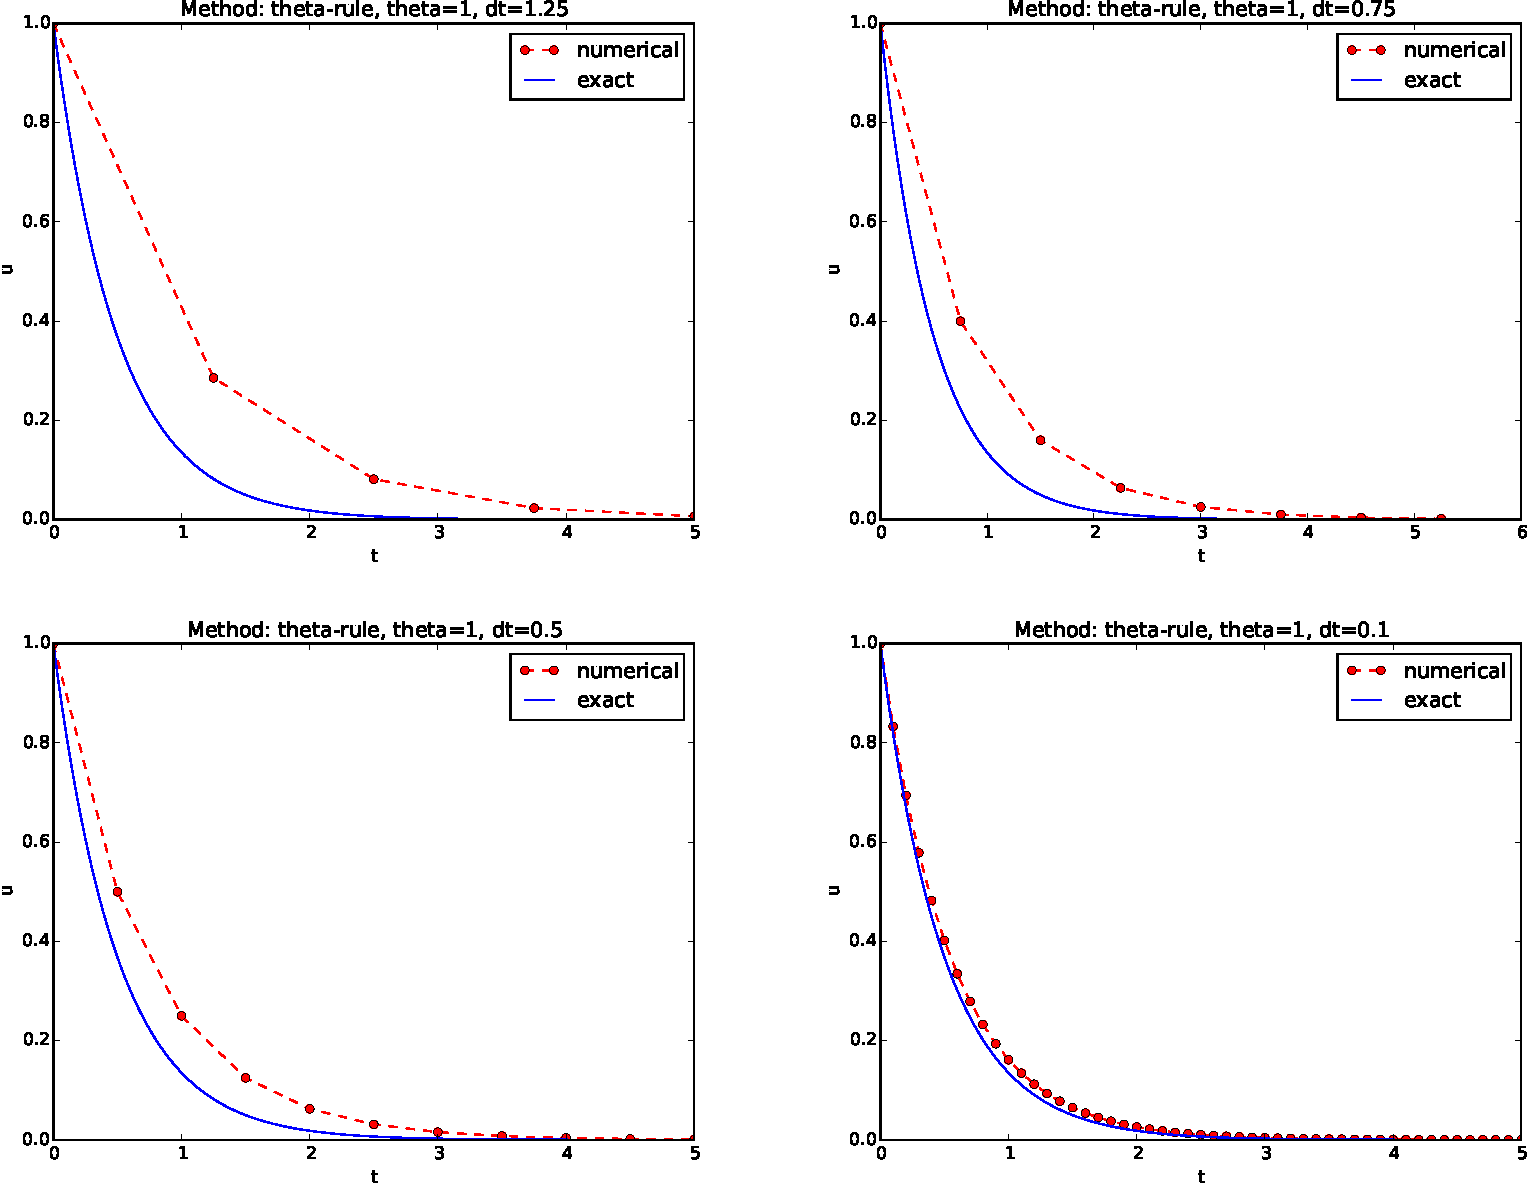
\includegraphics[width=1.1\linewidth]{fig-softeng/BE.pdf}}
  \caption{
  Illustration of the Backward Euler method for four time step values. \label{softeng1:experiments:fig:BE4a}
  }
\end{figure}
%\clearpage % flush figures softeng1:experiments:fig:BE4a


The appropriate ImageMagick commands are

\begin{Verbatim}[frame=lines,label=\fbox{{\tiny Terminal}},framesep=2.5mm,framerule=0.7pt,fontsize=\fontsize{9pt}{9pt}]
Terminal> montage -background white -geometry 100% -tile 2x \ 
          f1.png f2.png f3.png f4.png f.png
Terminal> convert -trim f.png f.png
Terminal> convert f.png -transparent white f.png
\end{Verbatim}
The first command mounts the four files in one, the next \texttt{convert} command
removes unnecessary surrounding white space, and the final \texttt{convert} command
makes the white background transparent.

High-quality montage of PDF files \texttt{f1.pdf},
\texttt{f2.pdf}, \texttt{f3.pdf}, and \texttt{f4.pdf} into \texttt{f.pdf} goes like

\begin{Verbatim}[frame=lines,label=\fbox{{\tiny Terminal}},framesep=2.5mm,framerule=0.7pt,fontsize=\fontsize{9pt}{9pt}]
Terminal> pdftk f1.pdf f2.pdf f3.pdf f4.pdf output tmp.pdf
Terminal> pdfnup --nup 2x2 --outfile tmp.pdf tmp.pdf
Terminal> pdfcrop tmp.pdf f.pdf
Terminal> rm -f tmp.pdf
\end{Verbatim}

\subsection{Running a program from Python}

The script for automating experiments needs to run the \texttt{model.py} program
with appropriate command-line options. Python has several tools for
executing an arbitrary command in the operating systems.
Let \texttt{cmd} be a string containing the desired command.
In the present case study, \texttt{cmd} could be \texttt{'python model.py --I 1 --dt 0.5 0.2'}.
The following code
executes \texttt{cmd} and loads the text output into a string \texttt{output}:

\begin{cod}{cbg_blue1}\begin{Verbatim}[numbers=none,fontsize=\fontsize{9pt}{9pt},baselinestretch=0.95,xleftmargin=2mm]
from subprocess import Popen, PIPE, STDOUT
p = Popen(cmd, shell=True, stdout=PIPE, stderr=STDOUT)
output, _ = p.communicate()

# Check if the execution was successful
failure = p.returncode
if failure:
    print 'Command failed:', cmd; sys.exit(1)
\end{Verbatim}
\end{cod}
\noindent
Unsuccessful execution usually makes it meaningless to continue
the program, and therefore we abort the program with \texttt{sys.exit(1)}.
Any argument different from 0 signifies to the computer's operating system
that our program stopped with a failure.


\begin{notice_mdfboxadmon}[Programming tip: use \protect\Verb!\_! for dummy variable.]
Sometimes we need to unpack tuples or lists in separate variables,
but we are not interested in all the variables. One example is

\begin{cod}{cbg_blue1}\begin{Verbatim}[numbers=none,fontsize=\fontsize{9pt}{9pt},baselinestretch=0.95,xleftmargin=2mm]
output, error = p.communicate()
\end{Verbatim}
\end{cod}
\noindent
but \texttt{error} is of no interest in the example above.
One can then use underscore \Verb!_! as variable name for the dummy
(uninteresting) variable(s):

\begin{cod}{cbg_blue1}\begin{Verbatim}[numbers=none,fontsize=\fontsize{9pt}{9pt},baselinestretch=0.95,xleftmargin=2mm]
output, _ = p.communicate()
\end{Verbatim}
\end{cod}
\noindent
Here is another example where we iterate over a list of three-tuples,
but the interest is limited to the second element in each three-tuple:

\begin{cod}{cbg_blue1}\begin{Verbatim}[numbers=none,fontsize=\fontsize{9pt}{9pt},baselinestretch=0.95,xleftmargin=2mm]
for _, value, _ in list_of_three_tuples:
    # work with value
\end{Verbatim}
\end{cod}
\noindent
\end{notice_mdfboxadmon}



We need to interpret the contents of the string
\texttt{output} and store
the data in an appropriate data structure for further processing.
Since the content is basically a table and will be transformed to
a spread sheet format, we let the columns in the table be represented
by lists in the program,
and we collect these columns in a dictionary whose keys are natural
column names: \texttt{dt} and the three values of $\theta$.
The following code translates the output of \texttt{cmd} (\texttt{output})
to such a dictionary of lists (\texttt{errors}):

\begin{cod}{cbg_blue1}\begin{Verbatim}[numbers=none,fontsize=\fontsize{9pt}{9pt},baselinestretch=0.95,xleftmargin=2mm]
errors = {'dt': dt_values, 1: [], 0: [], 0.5: []}
for line in output.splitlines():
    words = line.split()
    if words[0] in ('0.0', '0.5', '1.0'):  # line with E?
        # typical line: 0.0   1.25:    7.463E+00
        theta = float(words[0])
        E = float(words[2])
        errors[theta].append(E)
\end{Verbatim}
\end{cod}
\noindent

\subsection{The automating script}

We have now all the core elements in place to write the complete
script where we run
\texttt{model.py} for a set of $\Delta t$ values (given as positional
command-line arguments), make the error plot,
write the CSV file, and combine plot files as described above.
The complete code is listed below, followed by some explaining comments.

\begin{pro}{cbg_blue1}{bar_blue1}\begin{Verbatim}[numbers=none,fontsize=\fontsize{9pt}{9pt},baselinestretch=0.95,xleftmargin=2mm]
import os, sys, glob
import matplotlib.pyplot as plt

def run_experiments(I=1, a=2, T=5):
    # The command line must contain dt values
    if len(sys.argv) > 1:
        dt_values = [float(arg) for arg in sys.argv[1:]]
    else:
        print 'Usage: %s dt1 dt2 dt3 ...' %  sys.argv[0]
        sys.exit(1)  # abort

    # Run module file and grab output
    cmd = 'python model.py --I %g --a %g --T %g' % (I, a, T)
    dt_values_str = ' '.join([str(v) for v in dt_values])
    cmd += ' --dt %s' % dt_values_str
    print cmd
    from subprocess import Popen, PIPE, STDOUT
    p = Popen(cmd, shell=True, stdout=PIPE, stderr=STDOUT)
    output, _ = p.communicate()
    failure = p.returncode
    if failure:
        print 'Command failed:', cmd; sys.exit(1)

    errors = {'dt': dt_values, 1: [], 0: [], 0.5: []}
    for line in output.splitlines():
        words = line.split()
        if words[0] in ('0.0', '0.5', '1.0'):  # line with E?
            # typical line: 0.0   1.25:    7.463E+00
            theta = float(words[0])
            E = float(words[2])
            errors[theta].append(E)

    # Find min/max for the axis
    E_min = 1E+20; E_max = -E_min
    for theta in 0, 0.5, 1:
        E_min = min(E_min, min(errors[theta]))
        E_max = max(E_max, max(errors[theta]))

    plt.loglog(errors['dt'], errors[0], 'ro-')
    plt.loglog(errors['dt'], errors[0.5], 'b+-')
    plt.loglog(errors['dt'], errors[1], 'gx-')
    plt.legend(['FE', 'CN', 'BE'], loc='upper left')
    plt.xlabel('log(time step)')
    plt.ylabel('log(error)')
    plt.axis([min(dt_values), max(dt_values), E_min, E_max])
    plt.title('Error vs time step')
    plt.savefig('error.png');  plt.savefig('error.pdf')

    # Write out a table in CSV format
    f = open('error.csv', 'w')
    f.write(r'$\Delta t$,$\theta=0$,$\theta=0.5$,$\theta=1$' + '\n')
    for _dt, _fe, _cn, _be in zip(
        errors['dt'], errors[0], errors[0.5], errors[1]):
        f.write('%.2f,%.4f,%.4f,%.4f\n' % (_dt, _fe, _cn, _be))
    f.close()

    # Combine images into rows with 2 plots in each row
    image_commands = []
    for method in 'BE', 'CN', 'FE':
        pdf_files = ' '.join(['%s_%g.pdf' % (method, dt)
                              for dt in dt_values])
        png_files = ' '.join(['%s_%g.png' % (method, dt)
                              for dt in dt_values])
        image_commands.append(
            'montage -background white -geometry 100%' +
            ' -tile 2x %s %s.png' % (png_files, method))
        image_commands.append(
            'convert -trim %s.png %s.png' % (method, method))
        image_commands.append(
            'convert %s.png -transparent white %s.png' %
            (method, method))
        image_commands.append(
            'pdftk %s output tmp.pdf' % pdf_files)
        num_rows = int(round(len(dt_values)/2.0))
        image_commands.append(
            'pdfnup --nup 2x%d --outfile tmp.pdf tmp.pdf' % num_rows)
        image_commands.append(
            'pdfcrop tmp.pdf %s.pdf' % method)

    for cmd in image_commands:
        print cmd
        failure = os.system(cmd)
        if failure:
            print 'Command failed:', cmd; sys.exit(1)

    # Remove the files generated above and by model.py
    from glob import glob
    filenames = glob('*_*.png') + glob('*_*.pdf') + glob('tmp*.pdf')
    for filename in filenames:
        os.remove(filename)

if __name__ == '__main__':
    run_experiments(I=1, a=2, T=5)
    plt.show()
\end{Verbatim}
\end{pro}
\noindent

\index{Unix wildcard notation} \index{wildcard notation (Unix)}
\index{os.system@{\rm\texttt{os.system}}}

We may comment upon many useful constructs in this script:

\begin{itemize}
 \item \texttt{[float(arg) for arg in sys.argv[1:]]} builds a list of real numbers
   from all the command-line arguments.

 \item \Verb!['%s_%s.png' % (method, dt) for dt in dt_values]! builds a list of
   filenames from a list of numbers (\Verb!dt_values!).

 \item All \texttt{montage}, \texttt{convert}, \texttt{pdftk}, \texttt{pdfnup}, and \texttt{pdfcrop}
   commands for creating
   composite figures are stored in a
   list and later executed in a loop.

 \item \Verb!glob('*_*.png')! returns a list of the names of all files in the
   current directory where the filename matches the \href{{http://en.wikipedia.org/wiki/Glob_(programming)}}{Unix wildcard notation}
   \Verb!*_*.png! (meaning any text, underscore, any text, and then \texttt{.png}).

 \item \texttt{os.remove(filename)} removes the file with name \texttt{filename}.

 \item \texttt{failure = os.system(cmd)} runs an operating system command with
   simpler syntax than what is required by \texttt{subprocess} (but the output
   of \texttt{cmd} cannot be captured).
\end{itemize}

\noindent
\subsection{Making a report}
\label{softeng1:exper:report}

The results of running computer experiments are best documented in a
little report containing the problem to be solved, key code segments,
and the plots from a series of experiments. At least the part of the
report containing the plots should be automatically generated by the
script that performs the set of experiments, because in the script we
know exactly which input data that were used to generate a specific
plot, thereby ensuring that each figure is connected to the
right data. Take a look at \href{{http://tinyurl.com/nc4upel/_static/sphinx-cloud/}}{a sample report}  to see what we have in
mind.

\index{Word (Microsoft)}
\index{LibreOffice}
\index{OpenOffice}
\index{Google Docs}

\paragraph{Word, OpenOffice, GoogleDocs.}
Microsoft Word, its open source counterparts OpenOffice and
LibreOffice, along with GoogleDocs and similar online services are the
dominating tools for writing reports today. Nevertheless, scientific
reports often need mathematical equations and nicely typeset computer
code in monospace font. The support for mathematics and computer code
in the mentioned tools is in this author's view not on par with the
technologies based on \emph{markup languages} and which are addressed
below. Also, with markup languages one has a readable, pure text file
as source for the report, and changes in this text can easily be
tracked by version control systems like Git. The result is a very
strong tool for monitoring ``who did what when'' with the files,
resulting in increased reliability of the writing process. For
collaborative writing, the merge functionality in Git leads to safer
simultaneously editing than what is offered even by collaborative
tools like GoogleDocs.



\index{HTML}
\index{MathJax}

\paragraph{HTML with MathJax.}
HTML is the markup language used for web pages.  Nicely typeset computer
code is straightforward in HTML, and high-quality mathematical
typesetting is available using an extension to HTML called \href{{http://www.mathjax.org/}}{MathJax}, which allows formulas and equations to be
typeset with {\LaTeX} syntax and nicely rendered in web browsers, see
Figure~\ref{softeng1:exper:report:fig:mathjax}.  A relatively small
subset of {\LaTeX} environments for mathematics is supported, but the
syntax for formulas is quite rich. Inline formulas look like \Verb!\( u'=-au \)! while equations are surrounded by \Verb!$$! signs.  Inside such
signs, one can use \Verb!\[ u'=-au \]! for unnumbered equations, or
\Verb!\begin{equation}! and \Verb!\end{equation}! for
numbered equations, or \Verb!\begin{align}! and \Verb!\end{align}! for multiple
numbered aligned equations.  You need to be familiar with \href{{http://en.wikibooks.org/wiki/LaTeX/Mathematics}}{mathematical
typesetting in LaTeX} to write MathJax
code.

The file \href{{http://tinyurl.com/p96acy2/report_generation/exper1_html.py}}{\nolinkurl{exper1_mathjax.py}}
calls a script
\href{{http://tinyurl.com/p96acy2/exper1.py}}{\nolinkurl{exper1.py}}
to perform the numerical experiments and then runs Python
statements for creating an \href{{http://tinyurl.com/nc4upel/_static/report_mathjax.html.html}}{HTML file} with the source code for \href{{http://tinyurl.com/nc4upel/_static/report_mathjax.html}}{the scientific report}.


\begin{figure}[!ht]  % softeng1:exper:report:fig:mathjax
  \centerline{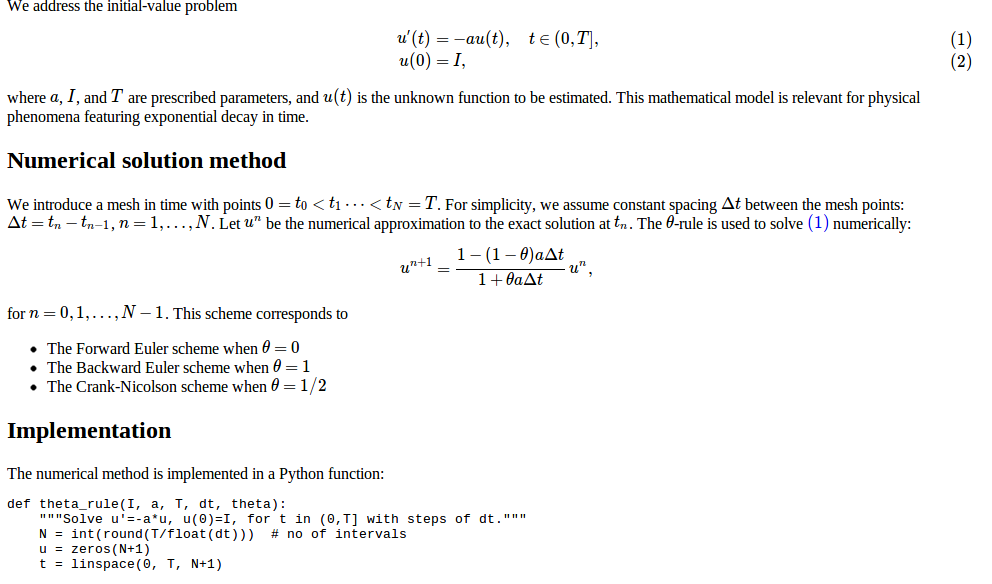
\includegraphics[width=0.9\linewidth]{fig-softeng/report_mathjax.png}}
  \caption{
  Report in HTML format with MathJax. \label{softeng1:exper:report:fig:mathjax}
  }
\end{figure}
%\clearpage % flush figures softeng1:exper:report:fig:mathjax


\index{LaTeX}

\paragraph{{\LaTeX}.}
% "http://en.wikibooks.org/wiki/LaTeX"

The \emph{de facto} language for mathematical typesetting and scientific
report writing is \href{{http://en.wikipedia.org/wiki/LaTeX}}{LaTeX}. A
number of very sophisticated packages have been added to the language
over a period of three decades, allowing very fine-tuned layout and
typesetting. For output in the \href{{http://tinyurl.com/nc4upel/_static/report.pdf}}{PDF format}, see Figure~\ref{softeng1:exper:report:fig:latex} for an example, {\LaTeX} is the
definite choice when it comes to \emph{typesetting quality}.
The {\LaTeX} language used to
write the reports has typically a lot of commands involving
\href{{http://tinyurl.com/nc4upel/_static/report.tex.html}}{backslashes and braces}, and many claim that
{\LaTeX} syntax is not particularly readable.  For output on the web via
HTML code (i.e., not only showing the PDF in the browser window), {\LaTeX}
struggles with delivering high quality typesetting. Other tools,
especially Sphinx, give better results and can also produce
nice-looking PDFs.  The file \href{{http://tinyurl.com/p96acy2/report_generation/exper1_latex.py}}{\nolinkurl{exper1_latex.py}} shows how to
generate the {\LaTeX} source from a program.


\begin{figure}[!ht]  % softeng1:exper:report:fig:latex
  \centerline{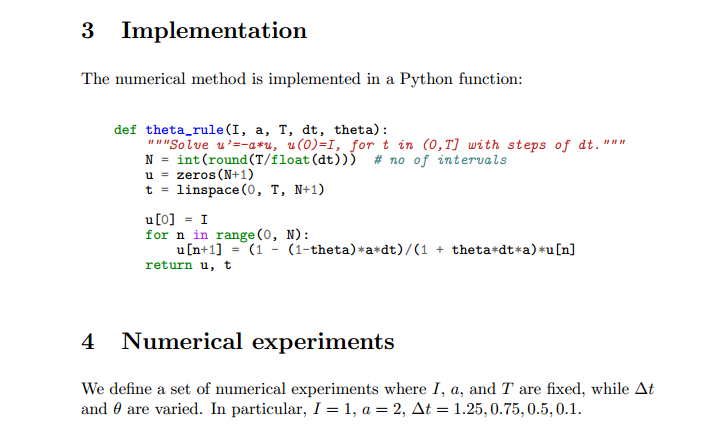
\includegraphics[width=0.9\linewidth]{fig-softeng/report_latexpdf.png}}
  \caption{
  Report in PDF format generated from {\LaTeX} source. \label{softeng1:exper:report:fig:latex}
  }
\end{figure}
%\clearpage % flush figures softeng1:exper:report:fig:latex


\index{Sphinx (typesetting tool)}

\paragraph{Sphinx.}
% give pointers to source pages

\href{{http://sphinx.pocoo.org/}}{Sphinx} is a typesetting language with
similarities to HTML and {\LaTeX}, but with much less tagging. It has
recently become very popular for software documentation and
mathematical reports. Sphinx can utilize {\LaTeX} for mathematical
formulas and equations. Unfortunately, the
subset of {\LaTeX} mathematics supported is less than in full MathJax (in
particular, numbering of multiple equations in an \texttt{align} type
environment is not supported).  The \href{{http://tinyurl.com/nc4upel/_static/report_sphinx.rst.html}}{Sphinx syntax} is an extension of
the reStructuredText language. An attractive feature of Sphinx is its
rich support for \href{{http://tinyurl.com/nc4upel/_static/sphinx-cloud/index.html}}{fancy layout of web pages}. In particular,
Sphinx can easily be combined with various layout \emph{themes} that give a
certain look and feel to the web site and that offers table of
contents, navigation, and search facilities, see Figure~\ref{softeng1:exper:report:fig:sphinx}.


\begin{figure}[!ht]  % softeng1:exper:report:fig:sphinx
  \centerline{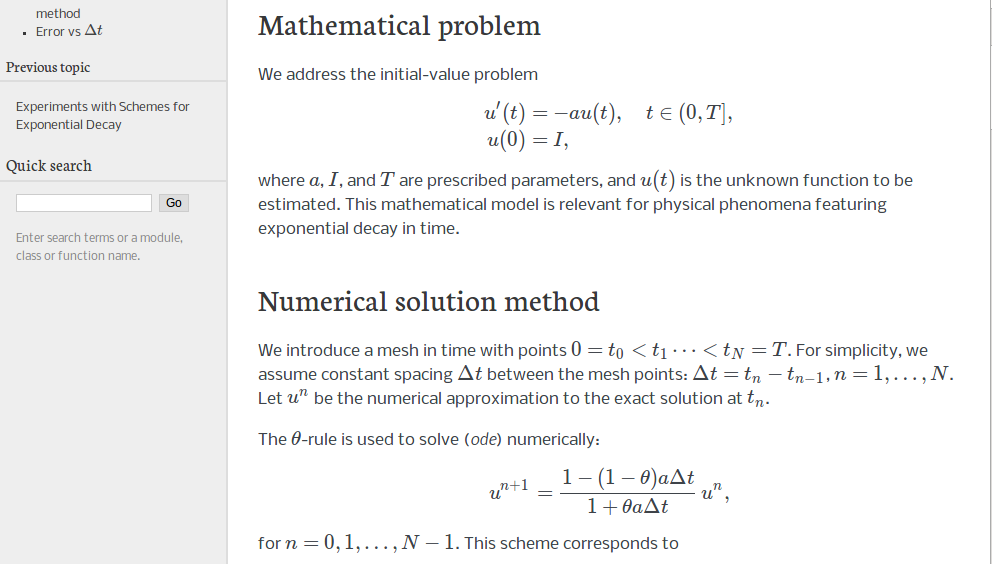
\includegraphics[width=0.9\linewidth]{fig-softeng/report_sphinx.png}}
  \caption{
  Report in HTML format generated from Sphinx source. \label{softeng1:exper:report:fig:sphinx}
  }
\end{figure}
%\clearpage % flush figures softeng1:exper:report:fig:sphinx


\index{Markdown}

\paragraph{Markdown.}
A recent, very popular format for easy writing of web pages is
\href{{http://daringfireball.net/projects/markdown/}}{Markdown}.
Text is written very much like one would do in email, using
spacing and special characters to naturally format the code
instead of heavily tagging the text as in {\LaTeX} and HTML.
With the tool \href{{http://johnmacfarlane.net/pandoc/}}{Pandoc} one
can go from Markdown to a variety of formats.
HTML is a common output format, but {\LaTeX}, epub, XML,
OpenOffice/LibreOffice, MediaWiki, and Microsoft Word are some other
possibilities. A Markdown version of our scientific
report demo is available as an IPython/Jupyter notebook (described next).

\index{IPython notebooks}
\index{Jupyter notebooks}

\paragraph{IPython/Jupyter notebooks.}
The \href{{http://ipython.org/notebook.html}}{IPython Notebook} is
a web-based tool where one can write scientific reports with live computer
code and graphics. Or the other way around: software can be equipped
with documentation in the style of scientific reports.
A slightly extended version of Markdown is used for writing text and
mathematics, and the \href{{http://tinyurl.com/nc4upel/_static/report.ipynb.html}}{source code of a notebook} is in json format.
The interest in the notebook has grown amazingly fast
over just a few years, and further development now takes place
in the \href{{https://jupyter.org/}}{Jupyter project}, which
supports a lot of programming languages for interactive notebook computing.
Jupyter notebooks are primarily live electronic documents, but they can be
printed out as PDF reports too.
A notebook version of our scientific report can be \href{{http://tinyurl.com/p96acy2/_static/report.ipynb}}{downloaded} and experimented with
or \href{{http://nbviewer.ipython.org/url/hplgit.github.com/teamods/writing_reports/_static/report.ipynb}}{just statically viewed} in a browser.

\paragraph{Wiki formats.}
A range of wiki formats are popular for creating notes on the web,
especially documents which allow groups of people to edit and add
content. Apart from \href{{http://www.mediawiki.org/wiki/MediaWiki}}{MediaWiki} (the wiki format used for
Wikipedia), wiki formats have no support for mathematical typesetting
and also limited tools for displaying computer code in nice ways.
Wiki formats are therefore less suitable for scientific reports compared
to the other formats mentioned here.

\index{DocOnce}

\paragraph{DocOnce.}
Since it is difficult to choose the right tool or format for writing a
scientific report, it is advantageous to write the content in a format
that easily translates to {\LaTeX}, HTML, Sphinx, Markdown,
IPython/Jupyter notebooks, and various wikis. \href{{https://github.com/hplgit/doconce}}{DocOnce} is such a tool. It is similar to
Pandoc, but offers some special convenient features for writing about
mathematics and programming.  The \href{{http://tinyurl.com/nc4upel/_static/report.do.txt.html}}{tagging is modest}, somewhere between
{\LaTeX} and Markdown.  The program \href{{http://tinyurl.com/p96acy2/exper1_do.py}}{\nolinkurl{exper1_do.py}} demonstrates how
to generate DocOnce code for a scientific report.
There is also a corresponding rich demo of the \href{{http://tinyurl.com/nc4upel/index.html}}{resulting reports} that can be made from
this DocOnce code.


% project with exploring instability (help with matplotlib contour plots, and maybe show such a plot)

\subsection{Publishing a complete project}
\label{softeng1:exper:github}

\index{replicability}

To assist the important principle of \emph{replicable} science,
a report documenting scientific investigations should be accompanied by
all the software and data used for the investigations so that others
have a possibility to redo the work and assess the qualify of the results.

One way of documenting a complete project is to make a directory tree
with all relevant files. Preferably, the tree is published at
some project hosting site like \href{{http://hplgit.github.com/teamods/bitgit/html/}}{Bitbucket or GitHub} so that others can download it
as a tarfile, zipfile, or clone the files directly using the Git version control
system.
For the investigations outlined in Section~\ref{softeng1:exper:report},
we can create a directory tree with files
\begin{cod}{cbg_blue1}\begin{Verbatim}[numbers=none,fontsize=\fontsize{9pt}{9pt},baselinestretch=0.95,xleftmargin=2mm]
setup.py
./src:
   model.py
./doc:
   ./src:
      exper1_mathjax.py
      make_report.sh
      run.sh
   ./pub:
      report.html
\end{Verbatim}
\end{cod}
\noindent
The \texttt{src} directory holds source code (modules) to be reused in other projects,
the \texttt{setup.py} script builds and installs such software,
the \texttt{doc} directory contains the documentation, with \texttt{src} for the
source of the documentation (usually written in a markup language)
and \texttt{pub} for published (compiled) documentation.
The \texttt{run.sh} file is a simple Bash script listing the \texttt{python} commands
we used to run \Verb!exper1_mathjax.py! to generate the experiments and
the \texttt{report.html} file.

% Point to DocOnce version


\section{Exercises}



% --- begin exercise ---
\begin{doconceexercise}
\refstepcounter{doconceexercisecounter}

\subsection*{Problem \thedoconceexercisecounter: Make a tool for differentiating curves}

\label{softeng1:exer:derivative}

Suppose we have a curve specified through a set
of discrete coordinates $(x_i,y_i)$, $i=0,\ldots,n$, where the $x_i$
values are uniformly distributed with spacing $\Delta x$: $x_i=\Delta x$.
The derivative of this curve, defined as a new curve with points
$(x_i, d_i)$, can be computed via finite differences:

\begin{align}
d_0 &= \frac{y_1-y_0}{\Delta x},\\ 
d_i &= \frac{y_{i+1}-y_{i-1}}{2\Delta x},\quad i=1,\ldots,n-1,\\ 
d_n &= \frac{y_n-y_{n-1}}{\Delta x}\tp
\end{align}


\subex{a)}
Write a function
\texttt{differentiate(x, y)} for differentiating a curve
with coordinates in the arrays \texttt{x} and \texttt{y}, using the
formulas above. The function should return the coordinate arrays
of the resulting differentiated curve.

\subex{b)}
Since the formulas for differentiation used here are only approximate,
with unknown approximation errors, it is challenging to construct
test cases. Here are three approaches, which should be implemented
in three separate test functions.

\begin{enumerate}
\item Consider a curve with three points and compute $d_i$, $i=0,1,2$,
   by hand. Make a test that compares the hand-calculated results with those
   from the function in a).

\item The formulas for $d_i$ are exact for points on
   a straight line, as all the $d_i$ values are then the same, equal to
   the slope of the line. A test can check this property.

\item For points lying on a parabola, the values for $d_i$, $i=1,\ldots,n-1$,
   should equal the exact derivative of the parabola. Make a test based on
   this property.
\end{enumerate}

\noindent
\subex{c)}
Start with a curve corresponding to $y=\sin(\pi x)$ and $n+1$
points in $[0,1]$. Apply \texttt{differentiate} four times and plot the
resulting curve and the exact $y=\sin\pi x$ for $n=6, 11, 21, 41$.

% Using a 2nd-order backward formula at x=1 does not improve the
% results much, one gets large errors at the end points.


\noindent Filename: \texttt{curvediff}.

\end{doconceexercise}
% --- end exercise ---




% --- begin exercise ---
\begin{doconceexercise}
\refstepcounter{doconceexercisecounter}

\subsection*{Problem \thedoconceexercisecounter: Make solid software for the Trapezoidal rule}

\label{softeng1:exer:integral:flat}

An integral

\[ \int_a^b f(x)dx \]
can be numerically approximated by the Trapezoidal rule,

\[ \int_a^b f(x)dx \approx \frac{h}{2}(f(a) + f(b)) + h\sum_{i=1}^{n-1} f(x_i),
\]
where $x_i$ is a set of uniformly spaced points in $[a,b]$:

\[ h = \frac{b-a}{n},\quad x_i=a + ih,\ i=1,\ldots,n-1\tp \]

Somebody has used this rule to compute the integral $\int_0^\pi \sin^2x\, dx$:

\begin{pro}{cbg_blue1}{bar_blue1}\begin{Verbatim}[numbers=none,fontsize=\fontsize{9pt}{9pt},baselinestretch=0.95,xleftmargin=2mm]
from math import pi, sin
np = 20
h = pi/np
I = 0
for k in range(1, np):
    I += sin(k*h)**2
print I
\end{Verbatim}
\end{pro}
\noindent


\subex{a)}
The ``flat'' implementation above suffers from serious flaws:

\begin{enumerate}
\item A general numerical algorithm (the Trapezoidal rule) is implemented
   in a specialized form where the formula for $f$ is inserted directly
   into the code for the general integration formula.

\item A general numerical algorithm is not encapsulated as a general
   function, with appropriate parameters, which can be reused
   across a wide range of applications.

\item The lazy programmer dropped the first terms in the general formula
   since $\sin(0)=\sin(\pi)=0$.

\item The sloppy programmer used \texttt{np} (number of points?) as variable for
   \texttt{n} in the formula and a counter \texttt{k} instead of \texttt{i}. Such small
   deviations from the mathematical notation are completely unnecessary.
   The closer the code and the mathematics can get, the easier it is
   to spot errors in formulas.
\end{enumerate}

\noindent
Write a function \texttt{trapezoidal} that fixes these flaws.
Place the function in a module \texttt{trapezoidal}.

\subex{b)}
Write a test function \Verb!test_trapezoidal!. Call the test function
explicitly to check that it works. Remove the call and run pytest
on the module:

\begin{Verbatim}[frame=lines,label=\fbox{{\tiny Terminal}},framesep=2.5mm,framerule=0.7pt,fontsize=\fontsize{9pt}{9pt}]
Terminal> py.test -s -v trapezoidal
\end{Verbatim}

% --- begin hint in exercise ---

\paragraph{Hint.}
Note that even if you know the value of the integral, you do not know
the error in the approximation produced by the Trapezoidal rule.
However, the Trapezoidal rule will integrate linear functions
exactly (i.e., to machine precision). Base a test function
on a linear $f(x)$.

% --- end hint in exercise ---

\subex{c)}
Add functionality such that we can compute $\int_a^b f(x)dx$ by providing
$f$, $a$, $b$, and $n$ as positional command-line arguments to the
module file:

\begin{Verbatim}[frame=lines,label=\fbox{{\tiny Terminal}},framesep=2.5mm,framerule=0.7pt,fontsize=\fontsize{9pt}{9pt}]
Terminal> python trapezoidal.py 'sin(x)**2' 0 pi 20
\end{Verbatim}
Here, $a=0$, $b=\pi$, and $n=20$.

Note that the \texttt{trapezoidal.py} file must still be a valid module file, so the
interpretation of command-line data and computation of the integral
must be performed from calls in a test block.

% --- begin hint in exercise ---

\paragraph{Hint.}
To translate a string formula on the command line, like \texttt{sin(x)**2},
into a Python function, you can wrap a function declaration around
the formula and run \texttt{exec} on the string to turn it into live Python code:

\begin{cod}{cbg_blue1}\begin{Verbatim}[numbers=none,fontsize=\fontsize{9pt}{9pt},baselinestretch=0.95,xleftmargin=2mm]
import math, sys
formula = sys.argv[1]
f_code = """
def f(x):
    return %s
""" % formula
exec(code, math.__dict__)
\end{Verbatim}
\end{cod}
\noindent
The result is the same as if we had hardcoded

\begin{cod}{cbg_blue1}\begin{Verbatim}[numbers=none,fontsize=\fontsize{9pt}{9pt},baselinestretch=0.95,xleftmargin=2mm]
from math import *

def f(x):
    return sin(x)**2
\end{Verbatim}
\end{cod}
\noindent
in the program. Note that \texttt{exec} needs the namespace
\Verb!math.__dict__!, i.e., all names in the \texttt{math} module, such that
it understands \texttt{sin} and other mathematical functions.
Similarly, to allow $a$ and $b$ to be \texttt{math} expressions like \texttt{pi/4}
and \texttt{exp(4)}, do

\begin{Verbatim}[frame=lines,label=\fbox{{\tiny Terminal}},framesep=2.5mm,framerule=0.7pt,fontsize=\fontsize{9pt}{9pt}]
a = eval(sys.argv[2], math.__dict__)
b = eval(sys.argv[2], math.__dict__)
\end{Verbatim}

% --- end hint in exercise ---

\subex{d)}
Write a test function for verifying the implementation of
data reading from the command line.

\noindent Filename: \texttt{trapezoidal}.

\end{doconceexercise}
% --- end exercise ---




% --- begin exercise ---
\begin{doconceexercise}
\refstepcounter{doconceexercisecounter}

\subsection*{Problem \thedoconceexercisecounter: Implement classes for the Trapezoidal rule}

\label{softeng1:exer:integral:flat2}

We consider the same problem setting as in Problem~\ref{softeng1:exer:integral:flat}. Make a module with a class \texttt{Problem}
representing the mathematical problem to be solved and a class
\texttt{Solver} representing the solution method.  The rest of the
functionality of the module, including test functions and reading data
from the command line, should be as in Problem~\ref{softeng1:exer:integral:flat}.
\noindent Filename: \Verb!trapezoidal_class!.

\end{doconceexercise}
% --- end exercise ---




% --- begin exercise ---
\begin{doconceexercise}
\refstepcounter{doconceexercisecounter}

\subsection*{Problem \thedoconceexercisecounter: Write a doctest and a test function}

\label{softeng1:exer:doctest1}

Type in the following program:

\begin{pro}{cbg_blue1}{bar_blue1}\begin{Verbatim}[numbers=none,fontsize=\fontsize{9pt}{9pt},baselinestretch=0.95,xleftmargin=2mm]
import sys
# This sqrt(x) returns real if x>0 and complex if x<0
from numpy.lib.scimath import sqrt

def roots(a, b, c):
    """
    Return the roots of the quadratic polynomial
    p(x) = a*x**2 + b*x + c.

    The roots are real or complex objects.
    """
    q = b**2 - 4*a*c
    r1 = (-b + sqrt(q))/(2*a)
    r2 = (-b - sqrt(q))/(2*a)
    return r1, r2

a, b, c = [float(arg) for arg in sys.argv[1:]]
print roots(a, b, c)
\end{Verbatim}
\end{pro}
\noindent


\subex{a)}
Equip the \texttt{roots} function with a doctest.
Make sure to test both real and complex roots.
Write out numbers in the doctest with 14 digits or less.

\subex{b)}
Make a test function for the \texttt{roots} function. Perform the
same mathematical tests as in a), but with different
programming technology.

\noindent Filename: \Verb!test_roots!.

\end{doconceexercise}
% --- end exercise ---




% --- begin exercise ---
\begin{doconceexercise}
\refstepcounter{doconceexercisecounter}

\subsection*{Problem \thedoconceexercisecounter: Experiment with tolerances in comparisons}

\label{softeng1:exer:tol}

When we replace a comparison \texttt{a == b}, where \texttt{a} and/or \texttt{b} are
\texttt{float} objects, by a comparison with tolerance, \texttt{abs(a-b) < tol},
the appropriate size of \texttt{tol} depends on the size of \texttt{a} and \texttt{b}.
Investigate how the size of \texttt{abs(a-b)} varies when \texttt{b} takes on
values $10^k$, $k=-5,-9,\ldots,20$ and \texttt{a=1.0/49*b*49}.
\noindent Filename: \texttt{tolerance}.

% Closing remarks for this Problem

\paragraph{Remarks.}
You will experience that if \texttt{a} and \texttt{b} are large, as they can be
in geophysical applications where lengths measured in meters can be of size
$10^6$ m, \texttt{tol} must be about $10^{-9}$, while \texttt{a} and \texttt{b} around unity can
have \texttt{tol} of size $10^{-15}$.


\end{doconceexercise}
% --- end exercise ---




% --- begin exercise ---
\begin{doconceexercise}
\refstepcounter{doconceexercisecounter}

\subsection*{Exercise \thedoconceexercisecounter: Make use of a class implementation}

\label{softeng1:exer:class:dts}

Implement the \Verb!experiment_compare_dt! function from \texttt{decay.py}
using class \texttt{Problem} and class \texttt{Solver} from
Section~\ref{softeng1:prog:se:class}.
The parameters \texttt{I}, \texttt{a}, \texttt{T}, the scheme name, and a series of
\texttt{dt} values should be read from the command line.
\noindent Filename: \Verb!experiment_compare_dt_class!.

\end{doconceexercise}
% --- end exercise ---




% --- begin exercise ---
\begin{doconceexercise}
\refstepcounter{doconceexercisecounter}

\subsection*{Problem \thedoconceexercisecounter: Make solid software for a difference equation}

\label{softeng1:exer:logistic}

We have the following evolutionary difference equation for the number
of individuals $u^n$ of a certain specie at time $n\Delta t$:

\begin{equation}
u^{n+1} = u^n + \Delta t\, r u^n\left(1 - \frac{u^n}{M^n}\right),
\quad u^0=U_0\tp
\label{softeng1:exer:logistic:eq}
\end{equation}
Here, $n$ is a counter in time, $\Delta t$ is time between time levels
$n$ and $n+1$ (assumed constant), $r$ is a net reproduction rate
for the specie,
and $M^n$ is the upper limit of the population that the environment can
sustain at time level $n$.
\noindent Filename: \texttt{logistic}.

\end{doconceexercise}
% --- end exercise ---


% !split


\bibliographystyle{plain}
\bibliography{../papers}

% ------------------- end of main content ---------------

% #ifdef PREAMBLE
\cleardoublepage\phantomsection  % trick to get correct link to Index
\printindex

\end{document}
% #endif

